%%%%%%%%%%%%%%%%%%%%%%%%%%%%%%%%%%%%%%%%%%%%%%%%%%%%%%%%%%%%%%%%%%%%%%%%%
%%   CHAPTER: UNIVERSAL COMPUTATION
%%%%%%%%%%%%%%%%%%%%%%%%%%%%%%%%%%%%%%%%%%%%%%%%%%%%%%%%%%%%%%%%%%%%%%%%%


\renewcommand{\chapterfolder}{universal_computation/}
\chapterimage{cover/universal_computation}
\chapter{Universal Computation}\label{chp:universal_computation}


\vspace*{-0.4in}
\epigraph{Becoming sufficiently familiar with something is a substitute for understanding it.}{John H. Conway}
\vspace*{0.4in}


\noindent At the end of Chapter~\ref{chp:periodic_circuitry}, we briefly introduced the concept of \textbf{computational universality}---the ability of Life (or other data manipulation rules in general) to simulate any computation that a computer can accomplish. It has been known since the early days of Life that it is computationally universal (also sometimes referred to as ``Turing complete'') \cite{Wain74,BCG82}. \index{Turing complete}\index{computational universality} However, the constructions that were used to originally demonstrate this fact were monstrously large and only \emph{mostly} pieced together. Actually constructing an explicit pattern that works as a universal computer that can be simulated in standard Life software still requires some additional work.

In this chapter, we dive into the details of one particularly flexible computation toolkit\footnote{Developed by Adam~P.~Goucher in 2009 and 2010 \cite{Gou10}.} that can be used to construct patterns that perform arbitrary computations, and even print the output of those computations in a font made up of blocks. For example, one of the major results of this chapter will be a pattern in Section~\ref{sec:pi_calc} that computes and prints the decimal digits of the mathematical constant $\pi$.


%%%%%%%%%%%%%%%%%%%%%%%%%%%%%%%%%%%%%%%%%%%%%%%%%%%%%%%%%%%%%%%%%%%%%%%%%
%%   SECTION: A COMPUTER IN LIFE
%%%%%%%%%%%%%%%%%%%%%%%%%%%%%%%%%%%%%%%%%%%%%%%%%%%%%%%%%%%%%%%%%%%%%%%%%
\section{A Computer in Life}\label{sec:computer_in_life}

What exactly does it mean to build a computer in the form of a Conway's Life pattern, anyway? To create a workable computational model in the form of a Life pattern, we need to construct patterns that implement a few different things:\smallskip

\begin{enumerate}
	\item[1)] We need mechanisms that can store information, preferably in the traditional binary form---zeroes and ones. We \emph{could} perfectly well break with tradition and build, say, a trinary computer based on memory mechanisms with three possible states, or a native decimal computer based on switches with ten different states, but binary two-state switches are much easier to design and to work with.\smallskip
	
	\item[2)] We need to be able to write programs made up of simple steps, or ``instructions''. Each step should have a specific effect on data stored in memory, and values stored in memory should be able to affect the flow of the program. After a conditional instruction, for example, if a given memory location contains ``1'' instead of ``0'', a completely different instruction might be the next to be executed.\smallskip
	
	\item[3)] Finally, we also need mechanisms that can represent arbitrarily complex programs. We have to store both the individual instruction steps, as well as the order in which they'll be executed (including the conditional ``jump'' instructions that depend on the current data stored in memory).\smallskip
\end{enumerate}

All of this may seem like a big leap in complexity from what we have covered so far, but most of the mechanisms that we need have already appeared in previous chapters. Our job in this chapter is to tie these known mechanisms together in the form of a working Life computer.


%%%%%%%%%%%%%%%%%%%%%%%%%%%%%%%%%%%%%%%%%%%%%%%%%%%%%%%%%%%%%%%%%%%%%%%%%
%%   SUBSECTION: A SLIDING BLOCK REGISTER
%%%%%%%%%%%%%%%%%%%%%%%%%%%%%%%%%%%%%%%%%%%%%%%%%%%%%%%%%%%%%%%%%%%%%%%%%
\subsection{A Sliding Block Register}\label{sec:sliding_block_register}

The first logic component that we construct will allow us to store and manipulate the value of a non-negative integer. While we could store the value of this integer in binary (and we will do exactly this in Section~\ref{sec:binary_register}), it will be easier for us to simply store it in the position of a single block. Indeed, we can move a block forward and backward via the block-moving operations that we used to make slide guns in Section~\ref{sec:slide_guns}, so we can use those operations to adjust the value that is stored in this device.

It is straightforward to use the techniques of Chapter~\ref{chp:stationary_circuitry} to build a stable conduit that turns a glider into the arrangement of three gliders from Figure~\ref{fig:synchronized_block_mover_5} that pushes a block diagonally away by $1$~cell. We call this an \texttt{INC}\index{INC} operation, since it corresponds to increasing the value that the block represents by $1$. We can similarly construct a conduit that turns a glider into the arrangement of two gliders from Figure~\ref{fig:synchronized_block_mover_4} that pulls the block diagonally closer by $1$~cell---a \texttt{DEC}\index{DEC} operation that decreases the value of the block by $1$.

However, in order for this mechanism to actually be useful in a computer, we need a way of reading its value (i.e., checking where the block is without disturbing it). To this end, we note that it suffices to be able to check whether or not the block is in the ``zero'' (\texttt{Z})\index{Z} position,\footnote{We could equally well call this the ``one'' position and store positive integers instead of non-negative integers, but it's more traditional to have the block's starting position be zero.} since we could repeatedly decrease the value of the block and perform that test after every decrement until we get a positive answer, and then increment the block back to its original position. Once we solve this problem of testing whether or not a block is in the ``zero'' position, we will have a memory device called a \textbf{sliding block register (SBR)}\index{sliding block register}\index{SBR|see {sliding block register}}.

The trick that we will use for performing this test is based on the $(2,1)$ block pull\index{(2,1) block pull} reaction that we first saw way back in Figure~\ref{fig:glider_block_move}. Indeed, this reaction is the one that happens when a glider just barely grazes a block, so we can position that glider so that it performs this $(2,1)$ block pull if the sliding block is in the ``zero'' position, and it simply passes by the block without any interaction at all if it is in any other position. In the latter case, we can simply use the unaffected glider as the ``non-zero'' (\texttt{NZ})\index{NZ} output of our test-if-zero (\texttt{TEST})\index{TEST} circuit. However, if the glider was destroyed by the $(2,1)$ block pull reaction (since the sliding block was in the ``zero'' position), we have some additional work to do: we have to arrange some circuitry so as to create a ``zero'' (\texttt{Z})\index{Z} output signal and also restore the moved sliding block to its original ``zero'' position.

Restoring the moved sliding block is simple enough---we just send another glider from the opposite direction so as to perform the opposite (2,1) block pull. However, we only want to send that glider if we failed to see an \texttt{NZ} output coming out of this \texttt{TEST} circuit. We thus need a second signal, split off from the \texttt{TEST} input, that is suppressed by a \texttt{NZ} output, but otherwise produces a \texttt{Z} output as well as a glider that resets the sliding block to the correct position. This kind of signal-logic thinking takes a while to get used to, but it's less complicated than it sounds. Figure~\ref{fig:sliding_block_schematic} displays a schematic that illustrates one way of handling the glider paths needed for this sliding block test-if-zero circuit and its two possible results.

\begin{figure}[!htb]
	\centering
	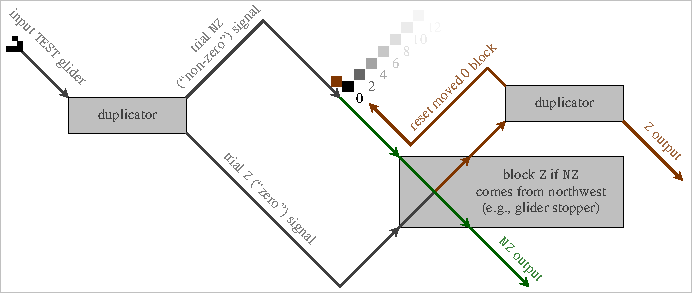
\includegraphics[width=\textwidth]{universal_computation/sliding_block_schematic.pdf}
	\caption{A schematic of a \texttt{TEST} circuit that tests whether or not a sliding block is in the ``zero'' (\texttt{Z}) position. If the block is in a non-zero (\texttt{NZ}) position then the trial \texttt{NZ} glider passes by without affecting it at all. Otherwise, the zero block is shifted via the $(2,1)$ block pull reaction, the trial \texttt{NZ} glider is destroyed, and the \texttt{Z} glider performs another $(2,1)$ block pull to put that zero block back in its original place.}\label{fig:sliding_block_schematic}
\end{figure}

We could then create a complete sliding block register by adding two additional inputs beyond just the \texttt{TEST} input:\smallskip

\begin{itemize}
	\item a \texttt{DEC} input that produces two gliders that are aimed at the sliding block as in Figure~\ref{fig:synchronized_block_mover_4}, so as to pull the block one cell closer, and\smallskip
	
	\item an \texttt{INC} input that produces the three gliders from Figure~\ref{fig:synchronized_block_mover_5} (two of which are the same as the gliders produced for the \texttt{DEC} operation), so as to push the block one cell farther away.\smallskip
\end{itemize}

A sliding block register with these three inputs could certainly be used in a Life computer, but we would have to be very careful never to write a program that might accidentally send a \texttt{DEC} signal when the block is already at the ``zero'' position. After all, if that ever happened then the \texttt{TEST} mechanism would fail catastrophically, because the glider that's supposed to graze the block so as to perform the (2,1) block pull reaction would instead run right into it.\footnote{By contrast, \texttt{INC} operations will never cause problems---it's always possible to move the block out by one more step to store the integer $n+1$ instead of $n$, so only \texttt{DEC} instructions are potentially dangerous.}

Our program could avoid this danger by always calling \texttt{TEST} first, and then only calling \texttt{DEC} if an \texttt{NZ} output comes back from \texttt{TEST}. However, a better option is to instead bake this idea right into the sliding block register itself, rather than relying on the programs that we write to do so. That is, we adjust the design of the sliding block register so that a \texttt{TEST} always happens just before a \texttt{DEC}. The circuit itself will then ignore the \texttt{DEC} input if the block is already at the \texttt{Z} position.

This slight redesign gives us an equally useful (and much safer!) sliding block register that has only two inputs: \texttt{INC} and \texttt{TEST}-then-\texttt{DEC}, which we abbreviate as \texttt{TDEC}.\index{TDEC} In this register, which is illustrated in Figure~\ref{fig:sliding_block_register}, there is no longer a way to send in a series of inputs that causes a catastrophic failure. Note that we have made the output \texttt{Z} and \texttt{NZ} lanes of this particular sliding block register transparent\index{transparent!lane} so that multiple registers can easily be placed side-by-side.

\begin{figure}[!htb]
	\centering
	\embedlink{sliding_block_register}{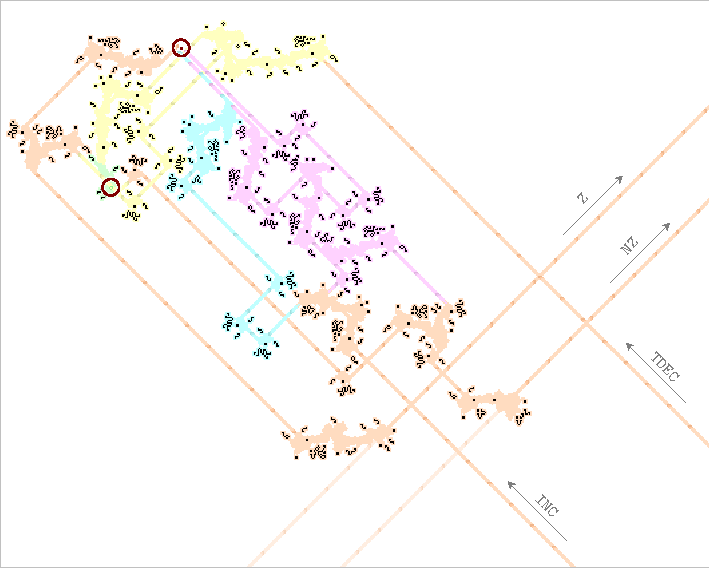
\includegraphics[width=\textwidth]{universal_computation/sliding_block_register.pdf}}
	\caption{A sliding block register. If a glider enters on the \texttt{INC} lane, the \bgbox{aquaback}{aqua} and \bgbox{magentaback}{magenta} conduits split it into three gliders that push the sliding block (circled in \bgbox{redback}{red} near the top) northwest by $1$ cell. If a glider enters on the \texttt{TDEC} lane, it enters the \texttt{TEST} circuit (the first half of which is highlighted in \bgbox{yellowback2}{yellow}). That \texttt{TEST} circuit uses a demultiplexer (highlighted in \bgbox{greenpastel}{green}) to switch the path of the glider---if the block is in the ``zero'' position then the glider passes through the demultiplexer to the northwest on the \texttt{Z} output path, and otherwise the demultiplexer creates a boat (circled in \bgbox{redback}{red} near the top-left) that redirects the glider to the northeast on the \texttt{NZ} output path. In the latter case, the \texttt{NZ} output glider is also fed into the \bgbox{magentaback}{magenta} conduit that creates two gliders to pull the sliding block $1$ cell southeast.}\label{fig:sliding_block_register}
\end{figure}


%%%%%%%%%%%%%%%%%%%%%%%%%%%%%%%%%%%%%%%%%%%%%%%%%%%%%%%%%%%%%%%%%%%%%%%%%
%%   SUBSECTION: ASSEMBLY CODE FOR A FINITE-STATE MACHINE
%%%%%%%%%%%%%%%%%%%%%%%%%%%%%%%%%%%%%%%%%%%%%%%%%%%%%%%%%%%%%%%%%%%%%%%%%
\subsection{Assembly Code for a Finite-State Machine}\label{sec:finite_state_machine}

We now have a mechanism that can store integer values, with two simple inputs (\texttt{INC} and \texttt{TDEC}) and two simple outputs (\texttt{Z} and \texttt{NZ}). Before delving into the details of how to position these registers on the Life plane to carry out computations, we first spend some time thinking about how to perform computations that only involve the operations corresponding to their input lanes---increasing or decreasing the value of some register, and checking whether or not a register is currently equal to zero.

To give a rough idea of how we could carry out a computation of this type, consider the task of just checking which of two registers contains a smaller value. We can solve this problem by repeatedly decrementing the value of the registers, and stopping once either of them is storing a value of \texttt{0}. Whichever one hits \texttt{0} first is determined to be the register that started off storing the smaller value. Pseudocode that implements this algorithm is provided by Pseudocode~\ref{alg:pseudocode_test_leq_or_ge}.

When we write pseudocode like this, we use labels like \texttt{U0}, \texttt{U1}, \texttt{U2}, $\ldots$ to denote the various registers used by the computer program.\footnote{The ``\texttt{U}'' stands for the word \textbf{unary}, since these sliding block registers stores integers in unary (i.e., the base-$1$ numeral system). We will see a different type of register that instead stores integers in binary a bit later, in Section~\ref{sec:binary_register}.} Also, for this particular pseudocode it is intended that the computer starts by executing the first line of code, then automatically moves to the following line and executes that, and so on---unless it encounters an instruction that tells it to \texttt{HALT} or jump to some other line of the program.

\begin{pseudocode}[!htb]
	\begin{algorithmic}[1]\small
		\State \texttt{if U0 = 0, jump to 6}
		\State \texttt{if U1 = 0, jump to 8}
		\State \texttt{decrement U0}
		\State \texttt{decrement U1}
		\State \texttt{jump to 1}
		\State \texttt{OUTPUT "U0 <= U1"}
		\State \texttt{HALT}
		\State \texttt{OUTPUT "U1 < U0"}
		\State \texttt{HALT}
	\end{algorithmic}
	\caption{Test which of the registers \texttt{U0} or \texttt{U1} contains a smaller value.}\label{alg:pseudocode_test_leq_or_ge}
\end{pseudocode}

Our next goal is to simplify and standardize our pseudocode so as to make it simpler to implement as a Life pattern. With this in mind, a \textbf{finite-state machine}\index{finite-state machine} is a model of computation in which the computer can be in one of a finite number of states at any given time, and its state can change based on inputs that it receives. We can implement a finite-state machine with $n$ possible states via a Life pattern that has a single glider traversing a set of $n$ parallel lanes connected by other circuitry.  At any given computer clock tick, the glider will be on exactly one of the ``state'' lanes. It will then run through structures that send gliders to various inputs of various register circuits, and also send a glider to the lane representing the next state in the program.

In order for our pseudocode to more accurately reflect this finite-state machine that our Life program will implement, we require $2$ additional things of all pseudocode that we write from this point forward:\smallskip

\begin{itemize}
	\item[1)] We include a ``jump'' instruction at the end of every single line. This corresponds to specifying exactly what state transition happens at each computer clock tick in the finite-state machine that we are implementing.\footnote{Our pseudocode, and the programming language that we will develop based on it, is thus one of the few examples of a language where execution does \emph{not} automatically proceed from one line to the next. For a more ``real-world'' example of such a language, see for example RPC-4000 machine code, as described in The Story of Mel: \httpurl{catb.org/jargon/html/story-of-mel.html}}\smallskip
	
	\item[2)] All conditional statements that we include are conditioned on whether the last output value received from a register was \texttt{Z} or \texttt{NZ}. We thus have to be careful to make sure that we always perform some task (like a \texttt{TDEC}) that returns a \texttt{Z} or \texttt{NZ} value immediately before jumping to a conditional statement.\smallskip
\end{itemize}

By making the changes outlined in points (1) and (2) above, our original Pseudocode~\ref{alg:pseudocode_test_leq_or_ge} is transformed into Pseudocode~\ref{alg:fsm_test_leq_or_ge}. These pseudocodes implement the same computational task (determining which of the two registers \texttt{U0} and \texttt{U1} is storing a smaller value), but the new pseudocode will be simpler for us to implement as a Life pattern. In particular, each line in Pseudocode~\ref{alg:fsm_test_leq_or_ge} now corresponds to a state in the finite-state machine that we will implement. This machine will start in the state of Line 1, and will move from state to state (i.e., line to line) until the algorithm has completed its work. Eventually either one output or the other will be sent out, and the program will reach its \texttt{HALT} state.

\begin{pseudocode}
	\begin{algorithmic}[1]\small
		\State \texttt{TDEC U0; jump to 2}
		\State \texttt{if return=Z then jump to 5, otherwise jump to 3}
		\State \texttt{TDEC U1; jump to 4}
		\State \texttt{if return=Z then jump to 6, otherwise jump to 1}
		\State \texttt{OUTPUT "U0 <= U1"; jump to 7}
		\State \texttt{OUTPUT "U1 < U0"; jump to 7}
		\State \texttt{HALT}
	\end{algorithmic}
	\caption{Test which of the registers \texttt{U0} or \texttt{U1} contains a smaller value---second version.}\label{alg:fsm_test_leq_or_ge}
\end{pseudocode}

We now refine this pseudocode even further and standardize it into what we call\index{APGsembly} \textbf{APGsembly code}---the programming language that we will use to write and compile computer programs in Life patterns.\footnote{The name ``APGsembly'' is a play on the word ``assembly'' (low-level code for programming computer instructions) and the initials of its author, Adam~P. Goucher. Indeed, APGsembly was used by Goucher to construct the original $\pi$ calculator in 2010.} In order to make the conditional statements of our pseudocode even easier to implement, we split each state of the finite state machine (i.e., our ``computer'') into two substates: one corresponding to the most recent return value being \texttt{Z}, and one corresponding to the most recent return value being \texttt{NZ}. These substates may result in completely different actions being taken and may cause the program to subsequently jump to completely different states (just as in a regular conditional statement).\footnote{In the actual Life implementation of the finite-state machine, this will mean that a glider will appear on one of two different parallel lanes during any given state, depending on whether the last output value received from a register was \texttt{Z} or \texttt{NZ}.}

Once we make the above change, we no longer really need logical instructions in our pseudocode at all: every program can be specified by listing what actions should be taken (e.g., \texttt{INC} or \texttt{TDEC}) when a particular state and substate is encountered, along with which state should then be jumped to next. See APGsembly~\ref{alg:apgsembly_test_leq_or_ge} for our first concrete example of APGsembly code---it implements the same ``does \texttt{U0} contain a smaller value than \texttt{U1}?'' test that we saw in Pseudocode~\ref{alg:fsm_test_leq_or_ge}.

\begin{apgsembly}
	\begin{algorithmic}\small
		\State \verb|# State    Input    Next state    Actions|
		\State \verb|# ---------------------------------------|
		\State \verb|INITIAL;   ZZ;      ID1;          TDEC U0|
		\State \verb|ID1;       Z;       ID2;          OUTPUT 0, HALT_OUT|
		\State \verb|ID1;       NZ;      ID2;          TDEC U1|
		\State \verb|ID2;       Z;       ID1;          OUTPUT 1, HALT_OUT|
		\State \verb|ID2;       NZ;      ID1;          TDEC U0|
	\end{algorithmic}
	\caption{APGsembly code to test which of the registers \texttt{U0} or \texttt{U1} contains a smaller value. An output value of \texttt{0} indicates that \texttt{U0 <= U1}, while an output value of \texttt{1} indicates that \texttt{U1 < U0}.}\label{alg:apgsembly_test_leq_or_ge}
\end{apgsembly}

On its surface, this APGsembly code looks quite different from the pseudocode that we saw earlier, so it is a good idea to trace through the program flow carefully until you are comfortable with the fact that it really does implement the exact same algorithm that we already saw. We now describe how APGsembly code is written, and how it differs from the pseudocode that we saw earlier:\smallskip

\begin{itemize}
	\item Line numbers from our pseudocode have been replaced by paired \texttt{ID} labels. Each state can have any alphanumeric ID label of our choosing, with the exception of the first, which is always called \texttt{INITIAL}.\footnote{Also, the \texttt{INITIAL} state should never be returned to later in a program's execution. It should be the first state, and \emph{only} the first state.} Using IDs like this instead of line numbers makes it much easier to manage our code---if we were to continue using line numbers instead of labels then we would have to update every single one of our ``jump'' instructions if we ever inserted a new line of code.\smallskip
	
	\item There are no longer any explicit ``if'' statements in the code, since each state (pair of lines sharing an ID label) acts implicitly as an ``if'' statement. \emph{If} the return value (from the previous action) is \texttt{Z}, perform the actions given on the first (\texttt{Z}) line; \emph{otherwise} perform the actions given in the second (\texttt{NZ}) line.\smallskip
	
	\item Sometimes, a particular state can only ever be reached by a \texttt{Z} input, so it does not need a corresponding \texttt{NZ} substate. In this case, the \texttt{NZ} substate can be omitted from the APGsembly code, and the \texttt{Z} substate is instead denoted by \texttt{ZZ} so that the compiler knows that the \texttt{NZ} omission was intentional. The \texttt{INITIAL} state is always assumed to have a \texttt{Z} input (just because the computer has to start in \emph{some} substate) and thus the first line of APGsembly code always starts with \texttt{INITIAL;ZZ}.\footnote{Similarly, if a state performs the exact same actions and jump operation regardless of whether it receives a \texttt{Z} or \texttt{NZ} return value, we can just list a single line for that state with \texttt{*} as its input value, instead of two otherwise identical lines with \texttt{Z} and \texttt{NZ} as their input values. We will not see an example of this in the main text, but it appears in Appendix~\ref{sec:appendix_apg}.}\smallskip
	
	\item Each line contains four items, separated by semicolons: state ID, input value, next state ID, and a comma-separated list of actions. The ``next state'' ID tells the program which state ID to jump to after performing the actions listed on the current line.\smallskip
	
	\item To make code easier to read, we can add comments to our code via lines that start with \texttt{\#} (so the first two lines of APGsembly~\ref{alg:apgsembly_test_leq_or_ge} do not actually affect what the code does, but just help us keep track of the four items on each line of code). For a similar reason, we can include any white space of our choosing between pieces of code, and empty lines between states if desired.\smallskip
	
	\item The \texttt{OUTPUT 0} and \texttt{OUTPUT 1} actions tell the Life computer to print out either a \texttt{0} or a \texttt{1} on the Life plane, in a font made up of blocks. We will see how this printing is actually done in Section~\ref{sec:decimal_printer}, but for now we note that by default this action can only print the digits \texttt{0}--\texttt{9} and periods (\texttt{.}), not more complicated expressions like ``\texttt{U0<=U1}''.\footnote{However, we will see in Section\ref{sec:decimal_printer} that this printing can, with slightly more work, be extended to any set of characters of our choosing.} The \texttt{HALT\_OUT} action stops the computer\footnote{For this reason, the ``next state'' provided in lines containing a \texttt{HALT\_OUT} action does not actually matter, since the computer never actually proceeds past that point.} (presumably because we are done our desired computation) and emits an output glider that could then be used by another pattern on the Life plane to detect that the computation finished.\smallskip
\end{itemize}

There are a few restrictions on what combinations of actions can be performed in a single line of APGsembly code. One of the reasons for this is that all actions on a particular line of APGsembly code are performed simultaneously, rather than sequentially. We should thus avoid single-line lists of actions like ``\texttt{TDEC U0, INC U0}'', for example, since the result of the \texttt{TDEC} may depend on whether or not the \texttt{INC} has already been completed, which is unpredictable. If the order of actions matters, they should be split into states on multiple different lines.

Furthermore, because of how these actions will be implemented in our Life computer (which we explore in the upcoming Section~\ref{sec:compiled_add_two_registers}), it is not possible to perform the same action more than once in a single substate (i.e., line of APGsembly). For example, if we want to increase the value of the register \texttt{U0} by \texttt{2}, it is tempting to use the list of actions ``\texttt{INC U0, INC U0}'' in a single line of APGsembly. However, this must be avoided---we should instead perform the first \texttt{INC U0}, then jump to another state, and then perform the next \texttt{INC U0}.

One final restriction comes from the fact that the return value from one line of APGsembly code dictates which substate of the next state is executed, so each line of APGsembly must contain exactly one action that produces a return value. If multiple actions were to produce a return value then it would not be clear which substate should be jumped to next, and if no action produced a return value then no substate would be jumped to and the computer would stop running altogether.\footnote{As a technical note, the \texttt{HALT\_OUT} action does not actually produce a return value (it does not need to, since we \emph{want} the computer to stop when it encounters \texttt{HALT\_OUT}). Instead, it is just a special action that bypasses the need for every line to have a return value.} So far, \texttt{TDEC} is the only action that we have introduced that produces a return value. Future sections will introduce some additional logic components that include value-returning actions, and a summary of these components and actions can be found by jumping ahead to Table~\ref{tab:universal_computation_components}. But first, let's take a look at what a compiled Life pattern arising from APGsembly code actually looks like.


%%%%%%%%%%%%%%%%%%%%%%%%%%%%%%%%%%%%%%%%%%%%%%%%%%%%%%%%%%%%%%%%%%%%%%%%%
%%   SECTION: A COMPILED APGSEMBLY PATTERN
%%%%%%%%%%%%%%%%%%%%%%%%%%%%%%%%%%%%%%%%%%%%%%%%%%%%%%%%%%%%%%%%%%%%%%%%%
\section{A Compiled APGsembly Pattern: Adding Registers}\label{sec:compiled_add_two_registers}

APGsembly code is specifically designed so that it can straightforwardly be compiled into a Life pattern.\footnote{Links to an APGsembly compiler, and some emulators that can be used to help debug APGsembly programs, can be found at \httpsurl{conwaylife.com/wiki/APGsembly}.} We now illustrate how this is done by constructing a Life computer that adds the values of two sliding block registers.

Our first step toward building such a computer is to write APGsembly code that implements the desired computational task. The code in APGsembly~\ref{alg:apgsembly_add_same_register} does the job nicely---it works by repeatedly decreasing the value of one register until it reaches a value of \texttt{0}, while simultaneously increasing the value of the other register every time. The only pieces of this APGsembly that we have not yet seen are the ``\texttt{\#COMPONENTS}'' and ``\texttt{\#REGISTERS}'' lines in the APGsembly's header. These lines are used to tell the APGsembly compiler which registers are used in the code,\footnote{``\texttt{U0-1}'' means that the code uses registers \texttt{U0} and \texttt{U1}. The ``\texttt{-}'' indicates a range (so ``\texttt{U0-2}'' would refer to registers \texttt{U0}, \texttt{U1}, and \texttt{U2}, for example).} and what the initial values of the registers should be, respectively. If a register is not initialized via the \texttt{\#REGISTERS} line, it starts with a value of \texttt{0}.

\begin{apgsembly}
	\begin{algorithmic}\small
		\State \verb|#COMPONENTS U0-1,HALT_OUT|
		\State \verb|#REGISTERS {'U0':7, 'U1':5}|
		\State \verb|# State    Input    Next state    Actions|
		\State \verb|# ---------------------------------------|
		\State \verb|INITIAL;   ZZ;      ID1;          TDEC U0|
		\State \verb|ID1;       Z;       ID1;          HALT_OUT|
		\State \verb|ID1;       NZ;      ID1;          TDEC U0, INC U1|
	\end{algorithmic}
	\caption{APGsembly code to add the value of \texttt{U0} to \texttt{U1}, and zero out \texttt{U0}. The \texttt{\#REGISTERS} line pre-loads the registers with the values \texttt{7} and \texttt{5}, respectively (so that after the computation completes, we will have \texttt{U0 = 0} and \texttt{U1 = 12}).}\label{alg:apgsembly_add_same_register}
\end{apgsembly}

While this code is quite simple (it's only $3$ lines long!), it illustrates an important oddity of APGsembly that we must keep in mind. Since \texttt{TDEC} is short for ``test and \emph{then} decrement'', it has the somewhat counterintuitive feature of giving a \texttt{Z} or \texttt{NZ} return value that is based on the value that was contained in it \emph{before} it was decremented. In particular, if we use a \texttt{TDEC} to decrement a register from 1 to 0, the return value will be \texttt{NZ}, not \texttt{Z}!

For this reason, APGsembly loops based on the \texttt{TDEC} action often require one more iteration than might be expected at first. If we want to decrement the value of a register from $n$ down to $0$, we have to call \texttt{TDEC} $n$ times. However, we then have to call it $1$ more time (which does not actually affect the value of the register, since it cannot decrease below $0$) in order to get a return value of \texttt{Z} instead of \texttt{NZ} and break out of the loop.

Since APGsembly code requires an action in the \texttt{INITIAL} state anyway before any loops are entered, we often put the extra \texttt{TDEC} command there (we did this in each of APGsembly~\ref{alg:apgsembly_test_leq_or_ge} and~\ref{alg:apgsembly_add_same_register}). The resulting code has the effect of decreasing the value of the register from $n$ to $n-1$, then looping from $n-1$ to $-1$, but with the register getting stuck at $0$ instead of actually decrementing all the way down to $-1$.

An actual Life pattern that implements the computation described by APGsembly~\ref{alg:apgsembly_add_same_register} is presented in Figure~\ref{fig:add_computer}. There is a lot going on in this pattern, so we now describe how it is built in some detail. This computer (and Life computers built from APGsembly in general) consists of three main parts: a \textbf{computer}\index{computer} (in the southeast), a \textbf{component stack}\index{component stack} (in the northwest), and a \textbf{clock gun} (in the north). We describe these three pieces one at a time.\index{component stack}\index{computer}\index{clock!gun}

\begin{figure}[!htb]
	\centering
	\embedlink{add_computer}{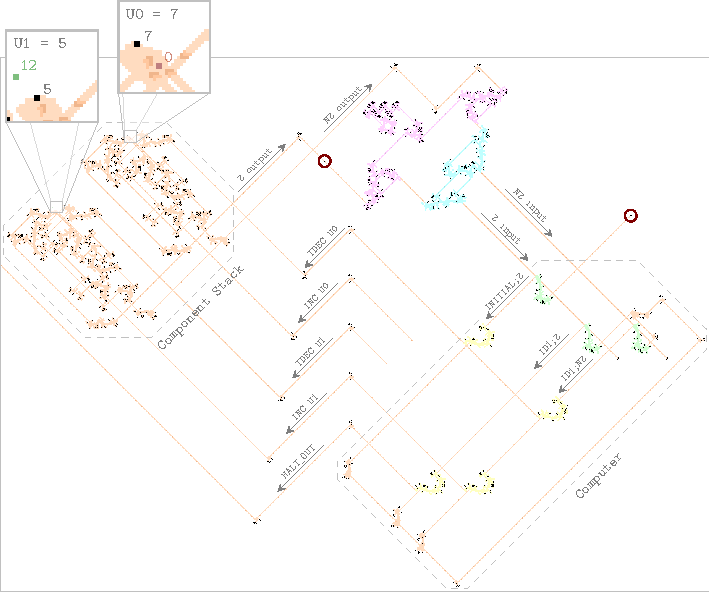
\includegraphics[width=\textwidth]{universal_computation/add_computer.pdf}}
	\caption{A compiled Life pattern that adds the values of the registers \texttt{U0} and \texttt{U1} (which have been pre-loaded with the values \texttt{7} and \texttt{5}, respectively), as in APGsembly~\ref{alg:apgsembly_add_same_register}. The registers at the west feed their output into the period~$2^{20}$ clock gun (highlighted in \bgbox{magentaback}{magenta} with two separate universal regulators---one for the \texttt{Z} path and another for the \texttt{NZ} path). The clock gun feeds a glider into a demultiplexer (highlighted in \bgbox{greenpastel}{green}) corresponding to the next substate of the computer (i.e., line of APGsembly). That demultiplexer then feeds into splitters (highlighted in \bgbox{yellowback2}{yellow}) corresponding to the actions in that line of APGsembly (the \texttt{INC U0} and \texttt{TDEC U1} lanes are disconnected from the computer because those actions are not called by any line of APGsembly~\ref{alg:apgsembly_add_same_register}). Finally, the duplicated gliders heading to the northwest feed back into the registers, and the duplicated glider heading to the southwest is reflected around the southeast end of the computer so as to activate the demultiplexer for its next state. The conduit highlighted in \bgbox{aquaback}{aqua} puts the \texttt{Z} or \texttt{NZ} glider coming from the clock gun on the correct input lane, and then produces an extra cleanup glider on each computer input lane so as to reset the demultiplexers. The two gliders circled in \bgbox{redback}{red} start the computation by activating the \texttt{INITIAL;Z} demultiplexer and then feeding a glider into it.}\label{fig:add_computer}
\end{figure}


\subsection{The Computer}

The computer is an implementation of a finite-state machine, so when it is at rest it is always in one of a finite number of different states, represented by a pair of demultiplexers that have a boat. Either a \texttt{Z} or an \texttt{NZ} signal will head southeast from the clock gun as a result of the computation performed in the computer's previous state. That glider will hit either the \texttt{Z} or the \texttt{NZ} demultiplexer and be reflected toward the southwest on a lane corresponding to exactly one specific line of APGsembly code.

If the computer is currently in state \texttt{ID1}, for example, then the two demultiplexers representing the \texttt{ID1} state both contain boats. If a \texttt{Z} signal comes in, the \texttt{Z} boat turns a glider onto the \texttt{ID1;Z} lane, and the \texttt{NZ} boat is cleaned up by a following glider. Conversely, if an \texttt{NZ} signal comes in, the \texttt{NZ} boat turns a glider onto the \texttt{ID1;NZ} lane, and the \texttt{Z} boat gets cleaned up instead.

The glider heading southwest then passes through one or more splitters---glider duplicators\index{splitter} that create a perpendicular glider while also sending another glider to continue along the exact same lane. As many splitters as we desire can thus be added along these lanes without changing the final destination of the southwest-travelling glider. Each splitter sends a glider on an output lane corresponding to an action from the current line of APGsembly code: \texttt{TDEC U0}, \texttt{INC U1}, and so on.

After going through the sequence of splitters, the southwest-bound glider hits a merge circuit---a reflector that is transparent to signals passing through it on its output lane. This implements the ``jump to'' part of each APGsembly line, and the transparency allows multiple lines of APGsembly to jump to the same state. Indeed, multiple merge circuits on the same northwest-to-southeast diagonal all produce gliders on the same lane, which are routed around to trigger the pair of demultiplexers for the next target state.\footnote{The computer in Figure~\ref{fig:add_computer} only has one path around its southern corner along which gliders can be reflected back into the demultiplexers. This is because every single line of APGsembly~\ref{alg:apgsembly_add_same_register} that generated that computer tells it to jump to the same state (\texttt{ID1}). We will see other computers shortly that can jump to multiple different states and thus have more glider paths down there.} The two boats then wait in the demultiplexer for the next \texttt{Z} or \texttt{NZ} signal from the clock.

As a technical implementation note, recall that the \texttt{INITIAL} state is always assumed to have a \texttt{Z} input. That \texttt{Z} input is hard-coded into the Life pattern in order to start the computation. The computer displayed in Figure~\ref{fig:add_computer} does not even have an \texttt{INITIAL;NZ} substate, since it would be impossible to reach anyway---recall that this is why the \texttt{INITIAL;Z} substate was listed as \texttt{INITIAL;ZZ} in APGsembly~\ref{alg:apgsembly_add_same_register}.


\subsection{The Component Stack}

In these calculator patterns, information is stored separately from the computer, in an array of ``components''. These components each have a finite number of inputs (called ``actions'' in APGsembly code) that can be used to manipulate or retrieve that information, and they potentially provide a single \texttt{Z}/\texttt{NZ} output bit. The first example that we have seen is the sliding block register, which has two action inputs (\texttt{INC Un} and \texttt{TDEC Un}) and the two standard outputs (\texttt{Z} and \texttt{NZ}). Since their output lanes are transparent, any number of sliding block registers \texttt{U0}, \texttt{U1}, \texttt{U2},$\ldots$ can be stacked side-by-side, and APGsembly code can \texttt{INC} or \texttt{TDEC} any one of them. If there are a lot of registers, the computer part of the pattern has to be stretched a little wider to accommodate spaces for more splitters. The computer has to be wide enough to hold two splitters for each sliding-block register---one for each \texttt{INC} action and one for each \texttt{TDEC} action.

Other components may have more or fewer action inputs. For example, we will see a binary register in Section~\ref{sec:binary_register} that has four actions: \texttt{INC Bn}, \texttt{TDEC Bn}, \texttt{READ Bn}, and \texttt{SET Bn}. New components could be designed to perform any logical function or store any amount of information that we might want; we will see an example of this in Section~\ref{sec:Osqrtlogt}, with the two-dimensional memory storage ``\texttt{B2D}'' component.

No matter how many components are added to the stack, they're all called in the same way, by a single glider travelling northwest on an ``action'' lane. Multiple actions can be triggered simultaneously, though each component may be activated at slightly different times depending on where it is placed in the stack. Since the precise timing of the actions depends heavily on how the computer and component stack are wired together, it is strongly recommended that a single line of code in APGsembly never triggers more than one action in a particular component. While it does not always cause problems, calling two simultaneous actions would cause many of the components that we consider here to fail. This problem can be avoided simply by calling the two incompatible actions from separate states (i.e., lines of APGsembly code).


\subsection{The Clock Gun}

Once a \texttt{Z} or \texttt{NZ} output signal is generated by the component stack, it is fed back into the computer in order to jump to the next state. However, we have to be slightly careful about when this glider arrives at the computer---we have to be sure that it does not arrive before the next state's demultiplexers are set in the computer (i.e., before the computer's glider has had a chance to go through the merge circuits and find its way all the way around the southern perimeter of the computer part of the pattern).\footnote{This is not much of a concern in the pattern from Figure~\ref{fig:add_computer} since the path around the computer is so short, but it becomes an issue for patterns with larger computers (i.e., patterns generated by more lines of APGsembly).}

To delay the component stack's output glider, we could simply extend the length of the path that it must follow back to the computer. However, we instead make use of a very high-period universal regulator.\index{universal regulator} The advantage of this method is that several pieces of the pattern then repeat predictably at the period of the universal regulator, which lets Life simulation software evolve it much quicker than it could if the glider timing was less regular. In particular, if we choose the universal regulator to align to some high power-of-two period, then Golly's \emph{HashLife}\index{HashLife} algorithm is able to evolve these patterns extremely quickly.\footnote{HashLife is an algorithm for simulating Life that was developed by Bill Gosper in 1984 \cite{Gos84}. It works by creating a lookup table that keeps track of how the $2^{n} \times 2^{n}$ center of certain repetitive $2^{n+1} \times 2^{n+1}$ chunks of a pattern evolve over $2^{n-1}$ generations. Since nothing outside of that $2^{n+1} \times 2^{n+1}$ square can affect its $2^{n} \times 2^{n}$ center within those $2^{n-1}$ generations, the results of that computation can simply be reused whenever that same square is encountered in the future.}

The universal regulator that we use\footnote{Constructed by Louis-François Handfield in April 2020.} is conceptually very simple. A stream of gliders coming from a gun of any (sufficiently large) period of our choosing comes in from the northeast and is split into two streams that destroy each other. However, if a glider comes in from the northwest then it is fed into a syringe and then one of the Herschel-to-boat factories from Figure~\ref{fig:H_to_boat}. The resulting boat suppresses a single glider from the gun's duplicated stream, letting a glider that is aligned to the period of that gun escape, as illustrated in Figure~\ref{fig:stable_universal_regulator}.

The gun that we attach to this universal regulator has period $2^{20}$, which we choose simply because it is a power of $2$ that is large enough to handle most of the calculators that we will construct in this chapter, but small enough that it can be simulated quickly in software like Golly. To actually construct this gun, we just do exactly what we did in Section~\ref{sec:large_glider_guns}: we attach period multipliers to another gun. This particular gun (displayed in Figure~\ref{fig:p2to_the_20_gun}) uses quadri-Snarks (see Exercise~\ref{exer:quadri_snark}) \index{quadri-Snark} attached to a p$256$ machine gun,\index{machine gun} but semi-Snarks could have been used instead at the expense of the gun being slightly larger.

\begin{figure}[!htb]
	\centering
	\begin{minipage}[t]{0.47\textwidth}
		\centering
		\embedlink{stable_universal_regulator}{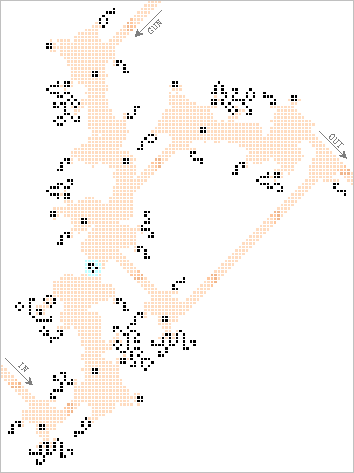
\includegraphics[width=0.9\textwidth]{universal_computation/stable_universal_regulator.pdf}}
		\caption{A stable universal regulator that works by having the input glider create a boat (highlighted in \bgbox{aquaback}{aqua}), which suppresses the glider on the southeast path and allows the northeast glider to escape.}\label{fig:stable_universal_regulator}
	\end{minipage}\hfill
	\begin{minipage}[t]{0.49\textwidth}
		\centering
		\patternimglink{0.135}{p2to_the_20_gun}
		\caption{A period~$2^{20}$ gun that works by using $6$ quadri-Snarks (highlighted in \bgbox{aquaback}{aqua} and \bgbox{magentaback}{magenta}) to repeatedly quadruple the period of a p$256$ machine gun.}\label{fig:p2to_the_20_gun}
	\end{minipage}
\end{figure}

The high-period universal regulator that results from stitching together Figures~\ref{fig:stable_universal_regulator} and~\ref{fig:p2to_the_20_gun} is called the \textbf{clock gun}, and it determines the speed at which the pattern computes whatever it has been programmed to compute. We think of the period of this clock gun as the clock speed of the computer, and one period of the regulator as one clock tick or computational cycle.\footnote{Some computations may take longer than one clock tick to complete, but that's okay. For example, if a sliding block register is storing an extremely large value then its sliding block will be extremely far away from the computer, so it will take a long time to \texttt{INC} or \texttt{TDEC}. In this case, the clock gun simply waits for one or more clock ticks until an output signal is received from the component stack.}

In summary, the calculator patterns that we compile from APGsembly work as follows:\smallskip

\begin{itemize}
	\item The computer in the southeast corner keeps track of the state and sends action commands to the component stack.\smallskip
	
	\item The action commands alter the contents of the components in the component stack, which serve as the computer's memory. Exactly one of these components then sends an output signal (glider) to the clock gun.\smallskip
	
	\item The clock gun regulates the glider signal coming from the component stack and feeds it back into the computer.
\end{itemize}


%%%%%%%%%%%%%%%%%%%%%%%%%%%%%%%%%%%%%%%%%%%%%%%%%%%%%%%%%%%%%%%%%%%%%%%%%
%%   SECTION: MULTIPLY TWO REGISTERS
%%%%%%%%%%%%%%%%%%%%%%%%%%%%%%%%%%%%%%%%%%%%%%%%%%%%%%%%%%%%%%%%%%%%%%%%%
\section{Multiplying and Reusing Registers}\label{sec:multiply_two_registers}

Now that we understand how to \emph{add} the value of two sliding block registers, we ramp up to the problem of \emph{multiplying} their values. One seemingly simple method of multiplying \texttt{U0} by \texttt{U1} and storing the result in \texttt{U2} would be to repeatedly add the register \texttt{U1} to \texttt{U2} a total of \texttt{U0} times. However, there is a slightly problem with this idea---our method of adding two registers from APGsembly~\ref{alg:apgsembly_add_same_register} zeroes out one of the registers while adding it to the other. Indeed, the only method that we have of looping over one register is based on \texttt{TDEC}ing it until it hits \texttt{0}, thus erasing the value that register contained.

To get around this problem, we introduce a temporary register into which we copy the value of one of the registers that we wish to loop over, and then we loop over that temporary register instead. In this particular case of setting \texttt{U2 = U0 * U1}, every time we add \texttt{U1} to \texttt{U2}, we do so by first copying \texttt{U1} to a new temporary register \texttt{U3} (zeroing out \texttt{U1} in the process), and then looping over \texttt{U3} so as to add it to each of \texttt{U1} \emph{and} \texttt{U2}. Pseudocode for carrying out this task, as well as the corresponding APGsembly code, is presented in APGsembly~\ref{apg:mult_unary_reg}.\footnote{After this code is executed, the value of \texttt{U1} is preserved, but the value of \texttt{U0} is not. If we want to preserve the value of \texttt{U0}, we can use \emph{another} temporary register (see Exercise~\ref{exer:universal_computation_mult_preserve_r0}).}

\begin{apgsembly}
	\centering
	\begin{minipage}[t]{.49\textwidth}
		\begin{algorithmic}[1]\small
			\State\texttt{TDEC U0}
			\State\texttt{if return value = Z:}
			\State\texttt{~~~~\# Loop U0 times, then halt.}
			\State\texttt{~~~~HALT}
			\State\texttt{else:}
			\State\texttt{~~~~\# Add U1 to U2 without erasing U1}
			\State\texttt{~~~~set U3 = U1}
			\State\texttt{~~~~set U1 = U3, U2 = U2 + U3}
			\State\texttt{end if}
			\State\texttt{jump to 1}
		\end{algorithmic}
	\end{minipage}\hfill{\color{gray}\vline}\hfill
	\begin{minipage}[t]{.49\textwidth}
		\begin{algorithmic}\tiny
			\State \verb|#COMPONENTS U0-3,HALT_OUT|
			\State \verb|#REGISTERS {'U0':7, 'U1':5}|
			\State \verb|# State    Input    Next state    Actions|
			\State \verb|# ---------------------------------------|
			\State \verb|INITIAL;   ZZ;      ID1;          TDEC U0|
			\State \verb||
			\State \verb|# Loop over U0, TDECing it until it hits 0, and then halt.|
			\State \verb|ID1;       Z;       ID1;          HALT_OUT|
			\State \verb|ID1;       NZ;      ID2;          TDEC U1|
			\State \verb||
			\State \verb|# Copy U1 into U3 while setting U1 = 0.|
			\State \verb|ID2;       Z;       ID3;          TDEC U3|
			\State \verb|ID2;       NZ;      ID2;          TDEC U1, INC U3|
			\State \verb||
			\State \verb|# Loop over U3, adding its value to U1 (restoring it) and U2.|
			\State \verb|ID3;       Z;       ID1;          TDEC U0|
			\State \verb|ID3;       NZ;      ID3;          TDEC U3, INC U1, INC U2|
		\end{algorithmic}
	\end{minipage}
	\caption{Pseudocode (left) and APGsembly code (right) to set \texttt{U2 = U0 * U1} and zero out \texttt{U0}. The register \texttt{U3} is used just temporarily (it starts and ends at the value of \texttt{0}) to store the value of \texttt{U1}. After this computation completes, the registers will have the values \texttt{U0 = 0}, \texttt{U1 = 5}, \texttt{U2 = 35}, and \texttt{U3 = 0}.}\label{apg:mult_unary_reg}
\end{apgsembly}

A Life pattern that was compiled from APGsembly~\ref{apg:mult_unary_reg} is displayed in Figure~\ref{fig:mult_computer}. This multiplication pattern has the same general shape and structure as the addition pattern from Figure~\ref{fig:add_computer}, but with slightly more of everything---$4$ sliding block registers instead of $2$, $7$ substates in the computer (corresponding to the $7$ lines of APGsembly code) instead of $3$, and so on. Perhaps the most notable change in this calculator pattern is that there are now $3$ glider lanes looping around the southern perimeter of the computer, whereas there was only $1$ such lane in Figure~\ref{fig:add_computer}. These extra lanes correspond to the fact that there are lines of APGsembly code in the multiplication program that jump to each of three different states (\texttt{ID1}, \texttt{ID2}, and \texttt{ID3}), whereas every line in the addition program jumped to the same state (\texttt{ID1}).

\begin{figure}[!htb]
	\centering
	\embedlink{mult_computer}{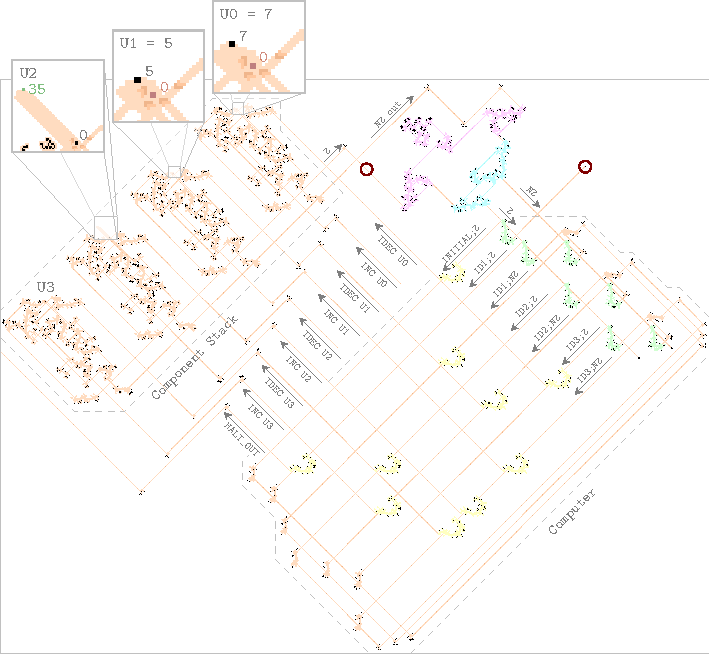
\includegraphics[width=\textwidth]{universal_computation/mult_computer.pdf}}
	\caption{A compiled Life pattern that multiplies the values of the registers \texttt{U0} and \texttt{U1} (which have been pre-loaded with the values \texttt{7} and \texttt{5}, respectively) and stores the result in \texttt{U2}, as in APGsembly~\ref{apg:mult_unary_reg}. The color scheme and general structure of this pattern is the same as in Figure~\ref{fig:add_computer}.}\label{fig:mult_computer}
\end{figure}

Just like we can multiply two registers via repeated addition, we can divide two registers via repeated subtraction. In particular, to compute the integer part of \texttt{U0 / U1} we can repeatedly subtract \texttt{U1} from \texttt{U0} until \texttt{U0 = 0}. The number of times that we were able to completely subtract \texttt{U1} is the integer part of \texttt{U0 / U1}, and the value that was contained in \texttt{U0} when we started our final subtraction is the remainder of that division. Implementing this division-by-subtraction algorithm in APGsembly is very similar to the multiplication-by-addition APGsembly~\ref{apg:mult_unary_reg}, so we leave it to Exercise~\ref{exer:division_by_subtraction}.

In fact, sliding block registers and the computational framework that we have introduced so far are already Turing complete---they can compute anything that can be computed. However, they are somewhat unwieldy to actually program to perform non-trivial computations, and they are not particularly interesting to look at. The remainder of this chapter is devoted to additional components that make computations in our Life patterns easier to implement, faster to perform, or simply more interesting to watch.


%%%%%%%%%%%%%%%%%%%%%%%%%%%%%%%%%%%%%%%%%%%%%%%%%%%%%%%%%%%%%%%%%%%%%%%%%
%%   SECTION: A BINARY REGISTER
%%%%%%%%%%%%%%%%%%%%%%%%%%%%%%%%%%%%%%%%%%%%%%%%%%%%%%%%%%%%%%%%%%%%%%%%%
\section{A Binary Register}\label{sec:binary_register}

One of the unfortunate features of sliding block registers is that the only actions they have available to them are addition and subtraction by \texttt{1}, so arithmetic operations involving large numbers stored in these registers take a long time to complete. For example, the addition code of APGsembly~\ref{alg:apgsembly_add_same_register} takes \texttt{U0+1} clock ticks to add the value of \texttt{U0} to \texttt{U1}, and the multiplication code of APGsembly~\ref{apg:mult_unary_reg} takes roughly \texttt{2 * U0 * U1} clock ticks to multiply \texttt{U0} by \texttt{U1}.\footnote{In fact, even the subtraction by \texttt{1} operation (i.e., \texttt{TDEC}) takes longer to complete if the value of the register is extremely large, since the sliding block takes longer to interact with and produce its return value when it is far away.}

While larger inputs leading to longer times to perform arithmetic operations is inevitable, we can save a lot of time by representing non-negative integers in a more efficient way than just as the position of a sliding block. While a sliding block register can be thought of as storing a non-negative integer in \textbf{unary}\index{unary} (i.e., the base-$1$ numeral system, in which each number is represented by tally marks or a distance from a fixed point), the register that we now introduce instead encodes non-negative integers in \textbf{binary} (i.e., the base-$2$ numeral system). Performing operations on such a register is somewhat more complicated, but it has the advantage of being much quicker because, for example, the non-negative integer $n$ can be stored in $\Theta(\log(n))$ space instead of $\Theta(n)$ space.%\footnote{Other bases larger than $2$ would also be quicker to work with than unary, but they would be even more complicated to implement.}

We call a register that stores a non-negative integer in this way a \textbf{binary register},\index{binary register} and the one that we make use of is displayed in Figure~\ref{fig:binary_register}. It uses block-moving shotguns similar to the ones in sliding block registers, except that they move a block~$6$ cells diagonally at a time instead of just~$1$. This wider spacing leaves room for additional reactions to place boats on one side of the sliding block. Every~$6$ cells along the sliding block's path is a designated bit location, which can contain either an empty space or a single boat, corresponding to the bits \texttt{0} and \texttt{1}, respectively.

\begin{figure}[!htb]
	\centering
	\embedlink{binary_register}{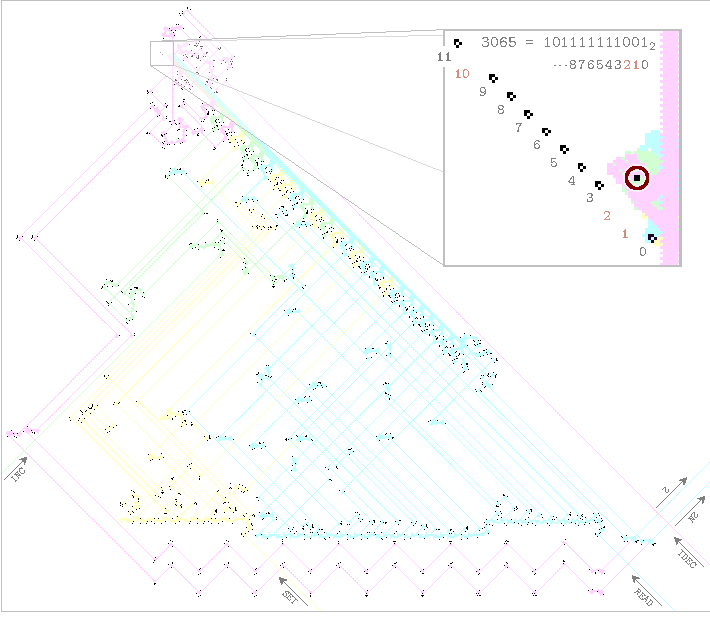
\includegraphics[width=\textwidth]{universal_computation/binary_register.pdf}}
	\caption{A binary register that uses a sliding block to keep track of the location of the read head (circled in \bgbox{redback}{red} in the zoom box at the ``\texttt{0}'' location) and boats to represent bits (shown here storing the value $3065 = 101111111001_2$). The sliding block and boat bits are manipulated by four different slow salvos corresponding to the register's four actions \texttt{INC}, \texttt{TDEC}, \texttt{READ}, and \texttt{SET}, which are generated by the circuitry highlighted in \bgbox{greenpastel}{green}, \bgbox{magentaback}{magenta}, \bgbox{aquaback}{aqua}, and \bgbox{yellowback2}{yellow}, respectively.}\label{fig:binary_register}
\end{figure}

The four actions available to this binary register are a bit more abstract than the actions of the sliding block register, since they work on the individual bits of the register rather than the value that those bits represent:\smallskip

\begin{itemize}
	\item An \texttt{INC}\index{INC} action moves the pointer block (called the \textbf{read head}\index{read head} of the register) to the next bit location, one step farther away.\smallskip
	
	\item A \texttt{TDEC}\index{TDEC} action moves the read head to the previous bit position (or keeps it in the same place if it's already at the zero position). This action also returns either \texttt{Z} or \texttt{NZ}, depending on whether or not the read head was already at the location of the least significant bit when this action was called.\footnote{This behavior is in complete analogy with the \texttt{TDEC} action for the sliding block register---it tests and \emph{then} it decrements (if possible). In fact, the \texttt{INC} and \texttt{TDEC} portions of the binary register from Figure~\ref{fig:binary_register} alone make up a sliding block register (they just manipulate the read head, not the boats that represent bits).}\smallskip
	
	\item A \texttt{READ}\index{READ} action sets the value of the bit at the current read head location to ``\texttt{0}''. This action returns either \texttt{Z} or \texttt{NZ}, depending on the original value of that bit.\smallskip
	
	\item Finally, a \texttt{SET}\index{SET} action places a ``\texttt{1}'' bit at the current read head location.\smallskip
\end{itemize}

Unlike a simple sliding block register, where there's no way to damage the mechanism by sending action signals to it, there are indeed ways to program a binary register that will cause it to explode catastrophically. In particular, if you send a \texttt{SET} action while there's already a \texttt{1} stored at the current read head location, it will cause irrecoverable damage. There's no built-in safety mechanism to prevent this, but this problem can easily be avoided by always sending a \texttt{READ} signal just before any \texttt{SET} signal.

We use \texttt{Bn} to denote the \texttt{n}-th binary register (where we start counting at \texttt{n = 0}), just like we use \texttt{Un} to denote the \texttt{n}-th sliding block register. To illustrate how to make use of these actions to perform bitwise operations, APGsembly~\ref{apg:store_139} shows how to store the value $139 = 10001011_2$ in a binary register \texttt{B0}.\footnote{The subscript ``$2$'' indicates that we are writing the number in binary.} Another way of storing the value $139$ in a binary register would be to change the appropriate line of the APGsembly header to \texttt{\#REGISTERS \{'B0':[0,'11010001']\}}. However, the header-based method only works if you want to set \texttt{B0} to $139$ at the start of the computation and not partway through it.

\begin{apgsembly}
	\begin{algorithmic}\small
		\State \verb|#COMPONENTS B0,NOP,HALT_OUT|
		\State \verb|#REGISTERS {}|
		\State \verb|# State    Input    Next state    Actions|
		\State \verb|# ---------------------------------------|
		\State \verb|INITIAL;   ZZ;      ID1;          SET B0, NOP|
		\State \verb|ID1;       ZZ;      ID2;          INC B0, NOP|
		\State \verb|ID2;       ZZ;      ID3;          SET B0, NOP|
		\State \verb|ID3;       ZZ;      ID4;          INC B0, NOP|
		\State \verb|ID4;       ZZ;      ID5;          INC B0, NOP|
		\State \verb|ID5;       ZZ;      ID6;          SET B0, NOP|
		\State \verb|ID6;       ZZ;      ID7;          INC B0, NOP|
		\State \verb|ID7;       ZZ;      ID8;          INC B0, NOP|
		\State \verb|ID8;       ZZ;      ID9;          INC B0, NOP|
		\State \verb|ID9;       ZZ;      ID10;         INC B0, NOP|
		\State \verb|ID10;      ZZ;      LSB1;         SET B0, NOP|
		\State
		\State \verb|# Move B0's read head back to its least significant bit.|
		\State \verb|LSB1;      ZZ;      LSB2;         TDEC B0|
		\State \verb|LSB2;      Z;       LSB2;         HALT_OUT|
		\State \verb|LSB2;      NZ;      LSB2;         TDEC B0|
	\end{algorithmic}
	\caption{APGsembly code for storing the value $139$ in the binary register \texttt{B0}, and then returning its read head to the least significant bit.}\label{apg:store_139}
\end{apgsembly}

This APGsembly also contains one new action that we have not yet seen: \texttt{NOP}.\index{NOP} This is an old standard programming abbreviation, short for ``\textbf{N}o \textbf{OP}eration''; it tells the computer not to change anything right now, but emit a \texttt{Z} return value anyway. It is typically used in conjunction with other actions that don't have a return value (\texttt{SET B0} and \texttt{INC B0} in this case), since exactly one action in every state's list of actions must return a value of either \texttt{Z} or \texttt{NZ}.\footnote{It may be tempting to merge multiple lines of APGsembly~\ref{apg:store_139} together so as to get rid of the \texttt{NOP} actions. For example, we might want to have an action list for a particular state that says something like \texttt{INC B0, INC B0, SET B0, NOP}. However, there are two problems with this: (1) we cannot call the same action twice in a single line of APGsembly (clock tick), and (2) it is not a good idea to perform two actions on the same register (\texttt{B0}) in the same clock tick. Indeed, it is not clear which one will be performed first (or even worse, they might interfere with each other and cause the register to self-destruct).}


%%%%%%%%%%%%%%%%%%%%%%%%%%%%%%%%%%%%%%%%%%%%%%%%%%%%%%%%%%%%%%%%%%%%%%%%%
%%   SECTION: A BINARY RULER
%%%%%%%%%%%%%%%%%%%%%%%%%%%%%%%%%%%%%%%%%%%%%%%%%%%%%%%%%%%%%%%%%%%%%%%%%
\subsection{A Binary Ruler}\label{sec:binary_ruler}

To illustrate how to perform some basic arithmetic operations with our binary register, consider the simple problem of increasing the value (i.e., the number that is stored in binary) of the register by~\texttt{1}. Unlike the sliding block register, there is no single action that performs this operation---we can only perform actions on one bit at a time, but increasing the value of a binary register by \texttt{1} may affect several of its bits due to carries.

Fortunately, since we are just increasing the value of the register by \texttt{1}, the carry bits are not difficult to take care of: we look for the least significant \texttt{0} bit and set it to \texttt{1}, and we set all bits that are less significant than it (which are necessarily currently equal to \texttt{1}) to \texttt{0}. Slightly more explicitly, we can increase the value of a binary register by \texttt{1} via the following procedure:\smallskip

\begin{enumerate}
	\item[1)] Start with the read head at the least significant bit and then proceed to step (2) below.\smallskip
	
	\item[2)] Read the value of the current bit (setting it equal to \texttt{0} in the process). If it equaled \texttt{0}, set it to \texttt{1} and then return the read head to the least significant bit. If it equaled \texttt{1}, move the read head to the next most significant bit (i.e., increase its position) and then return to step~(1).\smallskip
\end{enumerate}

This method is implemented in APGsembly~\ref{alg:apgsembly_binary_ruler}, which counts in binary by repeatedly adding \texttt{1} to the value of a binary register \texttt{B0}.\index{binary ruler}

\begin{apgsembly}
	\begin{algorithmic}\small
		\State \verb|#COMPONENTS B0,NOP|
		\State \verb|#REGISTERS {}|
		\State \verb|# State    Input    Next state    Actions|
		\State \verb|# ---------------------------------------|
		\State \verb|INITIAL;   ZZ;      CHECK1;       READ B0|
		\State
		\State \verb|## Determine whether the current bit equals 0 or 1.|
		\State \verb|# If it equals 0, set it to 1 and go to the least significant bit.|
		\State \verb|# If it equals 1, set it to 0 and go to the next most significant bit.|
		\State \verb|CHECK1;    Z;       LSB1;         SET B0, NOP|
		\State \verb|CHECK1;    NZ;      CHECK2;       INC B0, NOP|
		\State \verb|CHECK2;    ZZ;      CHECK1;       READ B0|
		\State
		\State \verb|# Move B0's read head back to its least significant bit.|
		\State \verb|LSB1;      ZZ;      LSB2;         TDEC B0|
		\State \verb|LSB2;      Z;       CHECK1;       READ B0|
		\State \verb|LSB2;      NZ;      LSB2;         TDEC B0|
	\end{algorithmic}
	\caption{APGsembly code for a \textbf{binary ruler}---a pattern that counts in binary.}\label{alg:apgsembly_binary_ruler}
\end{apgsembly}

One interesting feature of the pattern that results from compiling this APGsembly code (see Figure~\ref{fig:binary_ruler}) is that it exhibits a new type of slow growth that we have not yet seen. We explored patterns with slowly growing \emph{population} in Section~\ref{sec:irreg_guns}, but this pattern instead has a slowly growing \emph{bounding box}.\index{bounding box} In particular, its \textbf{diameter}\index{diameter} (i.e., its longest bounding box side length) in generation~$t$ is $\Theta(\log(t))$, since this is the rate at which new most significant bits are added to the end of the binary register.

\begin{figure}[!htb]
	\centering
	\embedlink{binary_ruler}{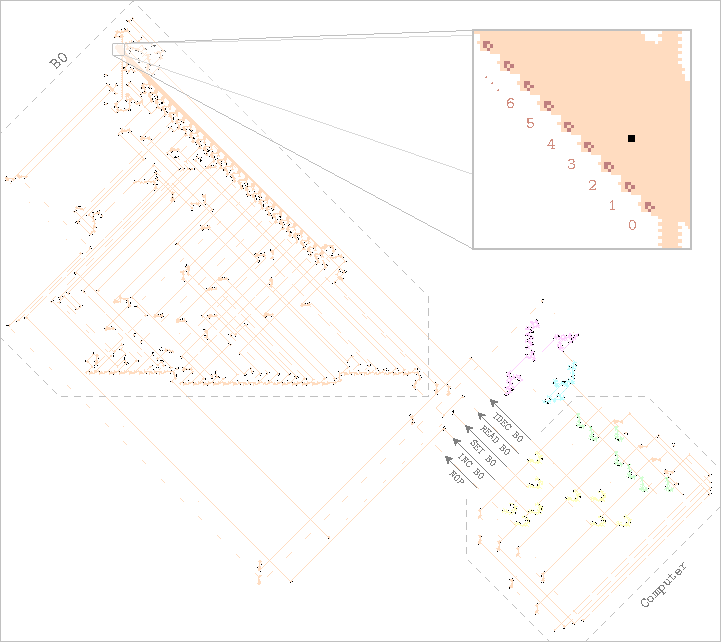
\includegraphics[width=\textwidth]{universal_computation/binary_ruler.pdf}}
	\caption{A \textbf{binary ruler} that counts in binary via APGsembly~\ref{alg:apgsembly_binary_ruler}. As a result, it grows very slowly, with its diameter in generation~$t$ being $\Theta(\log(t))$. Its component stack consists of just a single component---the binary register \texttt{B0}, which places boats that act as bits in the locations highlighted in \bgbox{redback}{red}.}\label{fig:binary_ruler}
\end{figure}

This diametric growth rate is much slower than any other unbounded pattern that we have seen so far (all of which have been $\Theta(t)$). We will return to this idea of patterns with slowly growing bounding boxes, and push it to its ultimate limit, in Section~\ref{sec:Osqrtlogt}.


%%%%%%%%%%%%%%%%%%%%%%%%%%%%%%%%%%%%%%%%%%%%%%%%%%%%%%%%%%%%%%%%%%%%%%%%%
%%   SECTION: BINARY ADDITION AND SUBTRACTION
%%%%%%%%%%%%%%%%%%%%%%%%%%%%%%%%%%%%%%%%%%%%%%%%%%%%%%%%%%%%%%%%%%%%%%%%%
\subsection{Addition, Subtraction, and Multiplication by 10}\label{sec:add_sub_and_mult10}\index{ADD component}\index{SUB component}

While addition and subtraction of values that are stored in sliding block (unary) registers is reasonably straightforward (refer back to Section~\ref{sec:compiled_add_two_registers}), these operations are more complicated for binary registers. Even just adding \texttt{1} to the value of a binary register and then resetting its read head makes use of seven lines of code (refer back to APGsembly~\ref{alg:apgsembly_binary_ruler}). The reason for the increase in complexity in this case is that when we add or subtract two binary numbers, we have to keep track of bits that are carried from one bit to the next, possibly many times in a row.

In order to make these arithmetic operations easier to perform, we introduce additional components that are custom-made for storing carry bits. In particular, the \texttt{ADD} and \texttt{SUB} components displayed in Figures~\ref{fig:add_component} and~\ref{fig:sub_component}, respectively, perform bitwise operations to assist in the addition and subtraction of binary registers.\footnote{These components were designed in 2009 or so, before the discovery of the Snark or the syringe. If desired, they could be rebuilt much smaller nowadays with modern Life technology.} The \texttt{ADD} component performs the addition of two bits, outputting the least significant bit of the addition and storing the carry bit in its own internal memory, and the \texttt{SUB} component similarly performs the subtraction of two bits while keeping track of the borrow bit.\footnote{Unlike the sliding block and binary registers, we only ever need one \texttt{ADD} or \texttt{SUB} component. In fact, every component that we see from this point on is limited to just a single copy per Life pattern---the sliding block and binary registers are the only components that we can use multiple copies of.}

\begin{figure}[!htb]
	\centering
	\begin{minipage}[t]{0.48\textwidth}
		\centering
		\embedlink{add_component}{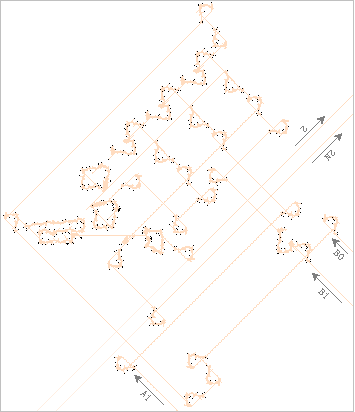
\includegraphics[width=\textwidth]{universal_computation/add_component.pdf}}
		\caption{The \texttt{ADD} component. To add up two bits \texttt{x} and \texttt{y} while respecting carry bits, input \texttt{A1} if \texttt{x = 1} (provide no input if \texttt{x = 0}) and then \texttt{By}.}\label{fig:add_component}
	\end{minipage}\hfill
	\begin{minipage}[t]{0.48\textwidth}
		\centering
		\embedlink{sub_component}{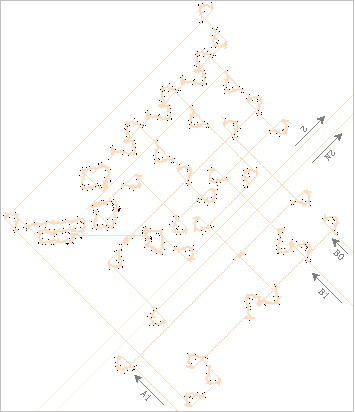
\includegraphics[width=\textwidth]{universal_computation/sub_component.pdf}}
		\caption{The \texttt{SUB} component. To subtract a bit \texttt{y} from \texttt{x} while respecting carry bits, input \texttt{A1} if \texttt{x = 1} (provide no input if \texttt{x = 0}) and then \texttt{By}.}\label{fig:sub_component}
	\end{minipage}
\end{figure}

More specifically, if we use \texttt{z} to denote the bit that is currently stored in the internal memory of the \texttt{ADD} component, then feeding two bits \texttt{x} and \texttt{y} into it returns a value of \texttt{(x + y + z) mod 2} and updates its memory to the value \texttt{(x + y + z)/2} (where we mean integer division here, so that this memory value is either \texttt{0} or \texttt{1}). This \texttt{ADD} component can then be used to add up the values stored in binary registers by repeatedly calling upon it to add up the least-significant bits of those registers, then their next-least-significant bits, and so on until all bits have been added.

However, this procedure only works if we know where the most significant bit is, so that we know when we can stop performing this bitwise addition. The binary registers themselves provide no such functionality---even if we find a million ``\texttt{0}'' bits in a row, there could always be a more significant ``\texttt{1}'' bit waiting to be found further on. For this reason, when performing bitwise arithmetic operations like addition and subtraction, we need to make use of a helper sliding block register that tells us (an upper bound of) how many bits the binary registers are making use of. The contents of this sliding block register needs to be updated as our computation proceeds to make sure that it always allocates enough bits of memory to the binary registers.

The way that the bit addition \texttt{x + y} is executed via APGsembly is that the pair of commands \texttt{ADD~Ax} and then \texttt{ADD~By} must be called (where we replace \texttt{x} and \texttt{y} by their actual binary values, as in \texttt{ADD B1}, for example).\footnote{Be careful: this means that \texttt{B0} and \texttt{B1} can be both components (as in \texttt{INC B0} or \texttt{READ B1}) and actions (as in \texttt{ADD B0}).} The \texttt{ADD Ax} command does not return an output (it just adds the input bit to the internal memory), but the \texttt{ADD By} command does (so it should always be used second). Furthermore, the \texttt{ADD A0} command is not actually implemented, since it does nothing---it does not return a value and also does not alter the internal memory.\footnote{This contrasts with the command \texttt{ADD B0}, which also does not alter the internal memory, but \emph{does} return a value. In particular, \texttt{ADD B0} returns the contents of the internal memory and then resets that memory to \texttt{0}.}

For example, to add binary registers containing the numbers $104 = 1101000_2$ and $57 = 111001_2$, we could perform the following sequence of actions in APGsembly (where we perform the ``\texttt{A}'' action in the top row and then the ``\texttt{B}'' action directly below it before moving left-to-right):
\begin{center}
	\begin{tabular}{llllllll}
		\leavevmode\hphantom{\texttt{ADD A0}} \ & \hphantom{\texttt{ADD A0}} \ & \hphantom{\texttt{ADD A0}} \ & \texttt{ADD A1} \ & \hphantom{\texttt{ADD A0}} \ & \texttt{ADD A1} \ & \texttt{ADD A1} \ & \hphantom{\texttt{ADD A0}} \\
		\texttt{ADD B1}, \ & \texttt{ADD B0}, \ & \texttt{ADD B0}, \ & \texttt{ADD B1}, \ & \texttt{ADD B1}, \ & \texttt{ADD B1}, \ & \texttt{ADD B0}, \ & \texttt{ADD B0}.
	\end{tabular}
\end{center}
Notice that these \texttt{ADD} actions are performed ``backwards'': they start from the least significant bits of the numbers that we are adding. Also, we need to append an extra \texttt{ADD B0} command at the very end to account for the fact that the sum may have one more bit than the summands.\footnote{Another reason that it is a good idea to call \texttt{ADD B0} after adding two registers is that it clears the internal memory of the \texttt{ADD} component.} These actions would return the outputs
\begin{center}
	\begin{tabular}{llllllll}
		\leavevmode\hphantom{\texttt{CD}}\texttt{NZ},\hphantom{\texttt{CD}} \ & \hphantom{\texttt{AB}}\texttt{Z},\hphantom{\texttt{CDE}} \ & \hphantom{\texttt{AB}}\texttt{Z},\hphantom{\texttt{CDE}} \ & \hphantom{\texttt{AB}}\texttt{Z},\hphantom{\texttt{CDE}} \ & \hphantom{\texttt{AB}}\texttt{Z},\hphantom{\texttt{CDE}} \ & \hphantom{\texttt{AB}}\texttt{NZ},\hphantom{\texttt{CD}} \ & \hphantom{\texttt{AB}}\texttt{Z},\hphantom{\texttt{CDE}} \ & \hphantom{\texttt{AB}}\texttt{NZ}\hphantom{\texttt{CD}}
	\end{tabular}
\end{center}
corresponding to the fact that $104 + 57 = 161 = 10100001_2$. Complete APGsembly that implements this addition of two binary registers is provided in APGsembly~\ref{alg:apgsembly_binary_add_sub}.

\begin{apgsembly}
	\centering
	\begin{minipage}[t]{.49\textwidth}
		\begin{algorithmic}\tiny
			\State \verb|#COMPONENTS B0-1,U0-2,ADD,NOP,HALT_OUT|
			\State \verb|#REGISTERS {'B0':[0,'0001011'], 'B1':[0,'100111'], 'U0':8}|
			\State \verb|# State    Input    Next state    Actions|
			\State \verb|# ---------------------------------------|
			\State \verb|INITIAL;   ZZ;      ADD1;         TDEC U0|
			\State \verb||
			\State \verb|# Copy U0 into U2, with the help of U1|
			\State \verb|ADD1;      Z;       ADD2;         TDEC U1|
			\State \verb|ADD1;      NZ;      ADD1;         TDEC U0, INC U1|
			\State \verb|ADD2;      Z;       ADD3;         TDEC U2|
			\State \verb|ADD2;      NZ;      ADD2;         TDEC U1, INC U0, INC U2|
			\State \verb||
			\State \verb|# Loop over U2 to add B1 to B0, one bit at a time.|
			\State \verb|ADD3;      Z;       ADD7;         TDEC B0|
			\State \verb|ADD3;      NZ;      ADD4;         READ B0|
			\State \verb|ADD4;      Z;       ADD5;         READ B1|
			\State \verb|ADD4;      NZ;      ADD5;         READ B1, ADD A1|
			\State \verb|ADD5;      Z;       ADD6;         ADD B0|
			\State \verb|ADD5;      NZ;      ADD6;         ADD B1, SET B1|
			\State \verb|ADD6;      Z;       ADD3;         TDEC U2, INC B0, INC B1|
			\State \verb|ADD6;      NZ;      ADD6;         SET B0, NOP|
			\State \verb||
			\State \verb|# Move the B0 and B1 read heads back to least significant bit.|
			\State \verb|ADD7;      Z;       ADD8;         TDEC B1|
			\State \verb|ADD7;      NZ;      ADD7;         TDEC B0|
			\State \verb|ADD8;      Z;       ADD8;         HALT_OUT|
			\State \verb|ADD8;      NZ;      ADD8;         TDEC B1|
		\end{algorithmic}
	\end{minipage}\hfill{\color{gray}\vline}\hfill
	\begin{minipage}[t]{.49\textwidth}
		\begin{algorithmic}\tiny
			\State \verb|#COMPONENTS B0-1,U0-2,SUB,NOP,HALT_OUT|
			\State \verb|#REGISTERS {'B0':[0,'0001011'], 'B1':[0,'100111'], 'U0':8}|
			\State \verb|# State    Input    Next state    Actions|
			\State \verb|# ---------------------------------------|
			\State \verb|INITIAL;   ZZ;      SUB1;         TDEC U0|
			\State \verb||
			\State \verb|# Copy U0 into U2, with the help of U1|
			\State \verb|SUB1;      Z;       SUB2;         TDEC U1|
			\State \verb|SUB1;      NZ;      SUB1;         TDEC U0, INC U1|
			\State \verb|SUB2;      Z;       SUB3;         TDEC U2|
			\State \verb|SUB2;      NZ;      SUB2;         TDEC U1, INC U0, INC U2|
			\State \verb||
			\State \verb|# Loop over U2 to subtract B1 from B0, one bit at a time.|
			\State \verb|SUB3;      Z;       SUB7;         TDEC B0|
			\State \verb|SUB3;      NZ;      SUB4;         READ B0|
			\State \verb|SUB4;      Z;       SUB5;         READ B1|
			\State \verb|SUB4;      NZ;      SUB5;         READ B1, SUB A1|
			\State \verb|SUB5;      Z;       SUB6;         SUB B0|
			\State \verb|SUB5;      NZ;      SUB6;         SUB B1, SET B1|
			\State \verb|SUB6;      Z;       SUB3;         TDEC U2, INC B0, INC B1|
			\State \verb|SUB6;      NZ;      SUB6;         SET B0, NOP|
			\State \verb||
			\State \verb|# Move the B0 and B1 read heads back to least significant bit.|
			\State \verb|SUB7;      Z;       SUB8;         TDEC B1|
			\State \verb|SUB7;      NZ;      SUB7;         TDEC B0|
			\State \verb|SUB8;      Z;       SUB8;         HALT_OUT|
			\State \verb|SUB8;      NZ;      SUB8;         TDEC B1|
		\end{algorithmic}
	\end{minipage}
	\caption{APGsembly code for adding (left) or subtracting (right) the binary register \texttt{B1} to/from \texttt{B0}. In both cases, the new value is stored in \texttt{B0} while the value of \texttt{B1} is unaffected. The number of bits allocated to the binary registers is stored in \texttt{U0}, and the registers \texttt{U1} and \texttt{U2} are only used temporarily (they start at, and are returned to, a value of \texttt{0}).}\label{alg:apgsembly_binary_add_sub}
\end{apgsembly}

Since the \texttt{ADD} component is somewhat technical and basically only has a single use, not much is lost if we do not actually understand its inner workings and just accept APGsembly~\ref{alg:apgsembly_binary_add_sub} as a black box that adds up two binary registers. Similarly, we do not go into any great depth in explaining the inner working of the \texttt{SUB} component. Instead, we just note that it does for subtraction exactly what the \texttt{ADD} component does for addition---it keeps track of the borrow bit (which is analogous to the carry bit for addition) and thus lets us subtract binary registers from each other one bit at a time. The resulting APGsembly code for subtracting one binary register from another one is also provided in APGsembly~\ref{alg:apgsembly_binary_add_sub}. Note that this code for subtracting \texttt{B1} from \texttt{B0} assumes that \texttt{B1 <= B0}; if you are unsure of which binary register is the smaller one then you should first compare them (see Exercise~\ref{exer:universal_computation_apgsembly_binary_compare}).

Now that we know how to add and subtract binary components, we can also multiply and divide them via the same tricks that we used for sliding block registers in Section~\ref{sec:multiply_two_registers} and Exercise~\ref{exer:division_by_subtraction}. That is, we simply add or subtract repeatedly (see Exercise~\ref{exer:universal_computation_apgsembly_multiply_binary}). However, doing so can be quite time-consuming when the registers store large values, so we now introduce one additional \index{MUL component} custom binary register arithmetic component---one that helps us multiply a binary register by $10$.\footnote{The reason for us making $10$ easier to multiply by (as opposed to any other fixed integer) is that multiplication by $10$ is a common operation when working with decimal numbers. In particular, we will make use of this multiplication-by-$10$ component to help us extract digits in the upcoming $\pi$~calculator in Section~\ref{sec:pi_calc}.}

This final new component is called \texttt{MUL}, which stores \emph{four} carry bits so that we can multiply a binary register by $10$ one bit at a time, just like the \texttt{ADD} and \texttt{SUB} components made use of a single memory bit to let us add and subtract binary registers one bit at a time.\footnote{The internal memory of these \texttt{ADD}, \texttt{SUB}, and \texttt{MUL} components is actually slightly more complicated than we have indicated. For example, the \texttt{ADD} component has \emph{two} bits of internal memory since between the \texttt{Ax} call (if any) and the \texttt{By} call, it tracks the carry bit and the \texttt{A} input value separately. Those values cannot be combined and stored in a single one-bit memory cell, because an internal \texttt{A0+(0 carry bit)} results in a different internal state than \texttt{A1+(1 carry bit)}, even though they both have a \texttt{Z} output.} The \texttt{MUL} component is displayed in Figure~\ref{fig:mul_component}, though it is not very enlightening to look at.\footnote{Even moreso than the binary register and \texttt{ADD} and \texttt{SUB} components, the \texttt{MUL} component could be made significantly smaller via modern machinery like Snarks and syringes.}

\begin{figure}[!htb]
	\centering
	\embedlink{mul_component}{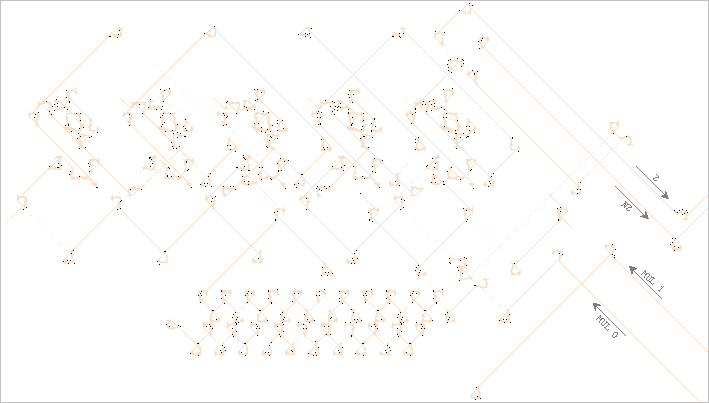
\includegraphics[width=\textwidth]{universal_computation/mul_component.pdf}}
	\caption{The \texttt{MUL} component, which keeps track of multiple carry bits so as to help us easily multiply a binary register by $10$.}\label{fig:mul_component}
\end{figure}

This component is called in APGsembly via the commands \texttt{MUL 0} and \texttt{MUL 1}, where the number after the name of the component refers to the current bit of the binary register that we are multiplying by $10$. For example, to multiply the number $26 = 11010_2$ by $10$, we could perform the following sequence of actions in APGsembly:
\begin{center}
	\texttt{MUL 0}, \ \ \texttt{MUL 1}, \ \ \texttt{MUL 0}, \ \ \texttt{MUL 1}, \ \ \texttt{MUL 1}, \ \ \texttt{MUL 0}, \ \ \texttt{MUL 0}, \ \ \texttt{MUL 0}, \ \ \texttt{MUL 0}.
\end{center}
These \texttt{MUL} actions also start from the least significant bit of the number that we are multiplying by $10$, just like the \texttt{ADD} and \texttt{SUB} actions. Also, we need to append enough \texttt{MUL 0} commands in order to retrieve the extra bits that the output will have. Four extra \texttt{MUL 0} commands always suffices, and these actions would return the outputs
\begin{center}
	\leavevmode\hphantom{\texttt{ABCD}}\texttt{Z}, \ \ \hphantom{\texttt{ABCD}}\texttt{Z}, \ \ \hphantom{\texttt{ABC}}\texttt{NZ}, \ \ \hphantom{\texttt{ABCD}}\texttt{Z}, \ \ \hphantom{\texttt{ABCD}}\texttt{Z}, \ \ \hphantom{\texttt{ABCD}}\texttt{Z}, \ \ \hphantom{\texttt{ABCD}}\texttt{Z}, \ \ \hphantom{\texttt{ABCD}}\texttt{Z}, \ \ \hphantom{\texttt{ABC}}\texttt{NZ},\hphantom{\texttt{ABCD}}
\end{center}
corresponding to the fact that $26 \times 10 = 260 = 100000100_2$.

We can thus now multiply a binary register by $10$ via approximately the same number of lines of APGsembly code as were required to add and subtract the values of binary registers. Complete APGsembly code for carrying out this multiplication is provided in APGsembly~\ref{alg:apgsembly_mul_ten}.

\begin{apgsembly}
	\begin{algorithmic}\small
		\State \verb|#COMPONENTS B0,U0-2,MUL,NOP,HALT_OUT|
		\State \verb|#REGISTERS {'B0':[0,'01011'], 'U0':9}|
		\State \verb|# State    Input    Next state    Actions|
		\State \verb|# ---------------------------------------|
		\State \verb|INITIAL;   ZZ;      MUL1;         TDEC U0|
		\State \verb||
		\State \verb|# Copy U0 into U2, with the help of U1|
		\State \verb|MUL1;      Z;       MUL2;         TDEC U1|
		\State \verb|MUL1;      NZ;      MUL1;         TDEC U0, INC U1|
		\State \verb|MUL2;      Z;       MUL3;         TDEC U2|
		\State \verb|MUL2;      NZ;      MUL2;         TDEC U1, INC U0, INC U2|
		\State \verb||
		\State \verb|# Loop over U2 to multiply B0 by 10, one bit at a time.|
		\State \verb|MUL3;      Z;       MUL6;         TDEC B0|
		\State \verb|MUL3;      NZ;      MUL4;         READ B0|
		\State \verb|MUL4;      Z;       MUL5;         MUL 0|
		\State \verb|MUL4;      NZ;      MUL5;         MUL 1|
		\State \verb|MUL5;      Z;       MUL3;         TDEC U2, INC B0|
		\State \verb|MUL5;      NZ;      MUL5;         SET B0, NOP|
		\State \verb||
		\State \verb|# Move the B0 read head back to its least significant bit.|
		\State \verb|MUL6;      Z;       MUL6;         HALT_OUT|
		\State \verb|MUL6;      NZ;      MUL6;         TDEC B0|
	\end{algorithmic}
	\caption{APGsembly code for multiplying the binary register \texttt{B0} by \texttt{10}. The number of bits allocated to \texttt{B0} is stored in \texttt{U0}, and the registers \texttt{U1} and \texttt{U2} are only used temporarily (they start at, and are returned to, a value of \texttt{0}). Compare with APGsembly~\ref{alg:apgsembly_binary_add_sub} for addition and subtraction.}\label{alg:apgsembly_mul_ten}
\end{apgsembly}


%%%%%%%%%%%%%%%%%%%%%%%%%%%%%%%%%%%%%%%%%%%%%%%%%%%%%%%%%%%%%%%%%%%%%%%%%
%%   SECTION: CHARACTER PRINTER
%%%%%%%%%%%%%%%%%%%%%%%%%%%%%%%%%%%%%%%%%%%%%%%%%%%%%%%%%%%%%%%%%%%%%%%%%
\section{A Character Printer}\label{sec:decimal_printer}\index{character printer}

We now demonstrate how to construct a component that is capable of printing any characters (e.g., digits or letters) of our choosing on the Life plane, in a font made up of blocks. Fortunately, we have already seen most of the reactions that we need to assemble a printer of this type. Very much along the same lines as the binary register of the previous section, our character printer will use a variant of slide gun technology to move a block that marks the current cursor position. We will also need a reaction that can use that cursor block to place another block nearby to serve as the pixels in printed characters (much like the read head block in the binary register can be used to place boats nearby to serve as bits in the register's memory).

In order to make our printer somewhat simpler to construct, we will have it move and position blocks via slow salvos like the ones that we introduced back in Section~\ref{sec:slow_salvo}. Doing this lets us not have to worry about the precise timing of the gliders that we use to move and duplicate blocks---we just have to position them correctly (which is trivial via an array of edge-shooting Herschel conduits). This is the same technique that we used to construct the binary register in Figure~\ref{fig:binary_register}, which has a long diagonal line of $26$~edge shooters along its northeast edge.

One particular salvo for placing a pixel block is displayed in Figure~\ref{fig:char_printer_place_pixel}. While this salvo is not quite slow (the first $3$ of its $7$ gliders must be synchronized, and the $4$th glider must have the correct mod~$8$ timing), it has the added benefit of being unidirectional.\footnote{We have already seen the slow portion of this salvo---the first slow glider is the $(2,1)$ block pull from Figure~\ref{fig:glider_block_move}, and the second and third gliders duplicate the block as in Figure~\ref{fig:slow_salvo_splitter}. The first four (synchronized) gliders just reposition the cursor block so that these later (slow) gliders, when duplicating the block, move it back to where it started.} Similarly, Figure~\ref{fig:char_printer_push_cursor} shows a 14-glider unidirectional slow salvo that pushes the cursor block 32 full diagonals farther away from the glider source. Importantly, this cursor-pushing reaction can be used regardless of whether or not the pixel-placing reaction was used, since the pixel is placed in a location that is never touched by the cursor-pushing reaction.

\begin{figure}[!htb]
	\centering
	\begin{subfigure}{\textwidth}
		\centering
		\embedlink{char_printer_place_pixel}{\vcenteredhbox{\patternimg{0.08}{char_printer_place_pixel_0}}} \vcenteredhbox{\genarrow{138}} \raisebox{-0.48\height}{\begin{tikzpicture}[scale=0.5, every node/.style={transform shape}]%
			\node[inner sep=0pt,anchor=south west] at (0,0) {\patternlink{char_printer_place_pixel}{\patternimg{0.16}{char_printer_place_pixel_138}}};
			
			\colorletternode{green}{5.07}{0.84}{1}
			\colorletternode{green}{5.75}{1.8}{2}
			\colorletternode{green}{3.6}{1.95}{3}
			\end{tikzpicture}} \vcenteredhbox{\gliderarrow{3}} \patternlink{char_printer_place_pixel}{\vcenteredhbox{\patternimg{0.08}{char_printer_place_pixel_141}}}
		\caption{A $7$-glider salvo that uses $4$ synchronized gliders and then $3$ slow gliders to create a far-away block, while only temporarily disturbing the target (cursor) block.}\label{fig:char_printer_place_pixel}
	\end{subfigure}\\[0.2cm]
	\begin{subfigure}{\textwidth}
		\centering
		\raisebox{-0.48\height}{\begin{tikzpicture}[scale=0.5, every node/.style={transform shape}]%
			\node[inner sep=0pt,anchor=south west] at (0,0) {\embedlink{char_printer_push_cursor}{\patternimg{0.234}{char_printer_push_cursor_0}}};
			
			\colorletternode{green}{4.55}{5.7}{1}
			\colorletternode{green}{3.7}{4.75}{2}
			\colorletternode{green}{3.05}{4.45}{3}
			\colorletternode{green}{0.55}{3.1}{4}
			\colorletternode{green}{1.9}{3.8}{5}
			\colorletternode{green}{2.9}{6.05}{6}
			\colorletternode{green}{2.7}{6.7}{7}
			\end{tikzpicture}} \vcenteredhbox{\gliderarrow{7}} \raisebox{-0.48\height}{\begin{tikzpicture}[scale=0.5, every node/.style={transform shape}]%
			\node[inner sep=0pt,anchor=south west] at (0,0) {\patternlink{char_printer_push_cursor}{\patternimg{0.234}{char_printer_push_cursor_7}}};
			
			\colorletternode{green}{6.05}{4.25}{1}
			\colorletternode{green}{5.4}{4.5}{2}
			\colorletternode{green}{4.85}{2.9}{3}
			\colorletternode{green}{4.8}{4.55}{4}
			\colorletternode{green}{3.2}{5}{5}
			\colorletternode{green}{3.05}{5.95}{6}
			\colorletternode{green}{3.1}{3.7}{7}
			\end{tikzpicture}} \vcenteredhbox{\gliderarrow{7}} \patternlink{char_printer_push_cursor}{\vcenteredhbox{\patternimg{0.117}{char_printer_push_cursor_14}}}
		\caption{A $14$-glider p$2$ slow salvo that pushes the target (cursor) block $32$~full diagonals away, while avoiding the location of the hypothetical printed pixel from~(a).}\label{fig:char_printer_push_cursor}
	\end{subfigure}
	\caption{Glider salvos that can be used to print block pixels at a separation of $32$~full diagonals.}\label{fig:char_printer_salvos}
\end{figure}

To create the salvos that implement these pixel-printing and cursor-moving operations, we just use stable circuitry like Snarks, syringes, and the edge-shooting Herschel conduits that we saw in Chapter~\ref{chp:stationary_circuitry}. If we want the next pixel in the current row to be empty, we just push the cursor block by creating the glider salvo from Figure~\ref{fig:char_printer_push_cursor}. If we want to print the next pixel in the current row, we instead create the salvo from Figure~\ref{fig:char_printer_place_pixel} and \emph{then} trigger the cursor-pushing mechanism. A device called a \textbf{row printer}\index{row printer} that implements both of these operations is displayed in Figure~\ref{fig:row_printer}.

\begin{figure}[!htb]
	\centering
	\embedlink{row_printer}{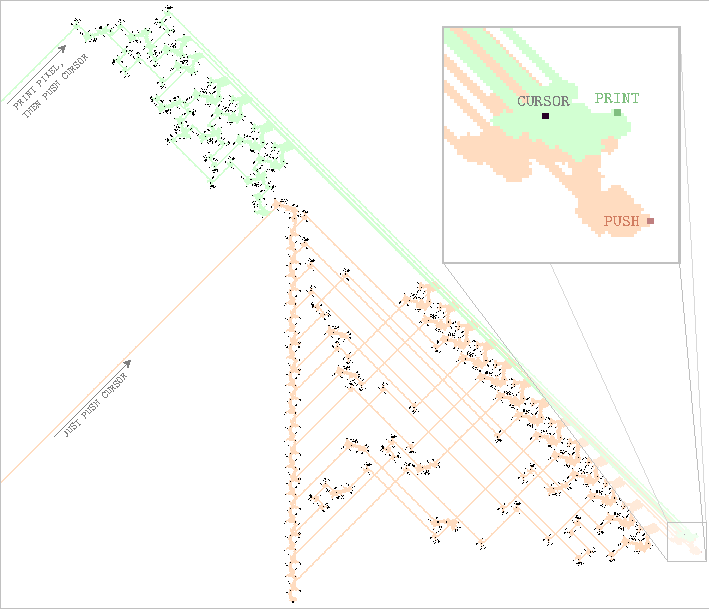
\includegraphics[width=\textwidth]{universal_computation/row_printer.pdf}}
	\caption{A \textbf{row printer} that can be used to either push a cursor block forward by $32$ full diagonals (highlighted in \bgbox{orangeback2}{orange}), or print a pixel block (highlighted in \bgbox{greenpastel}{green}) and \emph{then} push the cursor block.}\label{fig:row_printer}
\end{figure}

This row printer lets us easily print an arbitrary sequence of pixels (blocks) along a single (northwest-to-southeast diagonal) row. To construct a more general printer that lets us print characters that are several pixels tall, we simply use multiple row printers---one cursor block and one row printer per pixel of height in the characters. For example, if we wish to print characters that are $10$~pixels tall, we use $10$ cursor blocks that are offset from each other diagonally in the southwest-to-northeast direction, and we aim a separate row printer at each of them.

The end result of using multiple row printers in this way is that each row always advances its cursor block by the same distance ($32$ full diagonals), regardless of whether or not a pixel has been placed in that row. Instructions for which pixels to print in each row (and thus which characters to print overall) can be encoded straightforwardly in circuitry that sends a glider into the appropriate input slot of each row printer. To illustrate this idea, Figure~\ref{fig:abracadabra_printer} presents a pattern that is capable of printing the characters \texttt{A}, \texttt{B}, \texttt{C}, \texttt{D}, and \texttt{R} in a font made up of blocks, and which has had $11$ glider signals fed into it, instructing it to print the word ``\texttt{ABRACADABRA}''.

\begin{figure}[!htb]
	\centering
	\embedlink{abracadabra_printer}{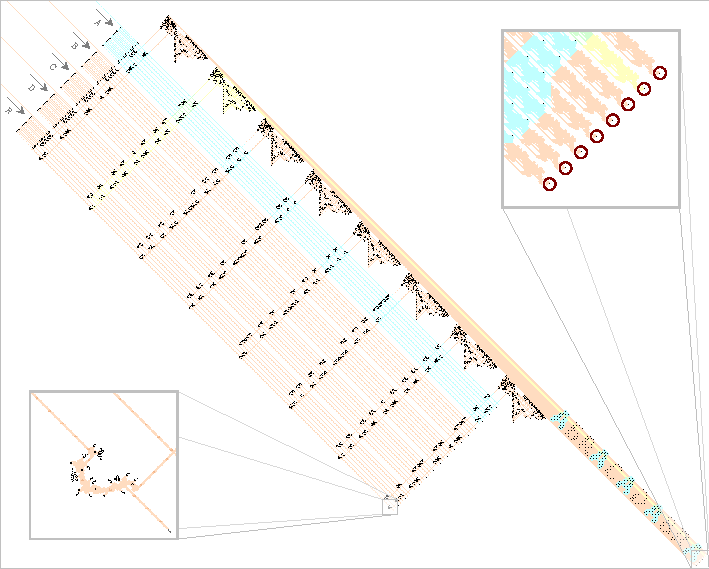
\includegraphics[width=\textwidth]{universal_computation/abracadabra_printer.pdf}}
	\caption{A printer with five input glider lanes that direct it to print one of the letters \texttt{A}, \texttt{B}, \texttt{C}, \texttt{D}, or \texttt{R} in a font made up of blocks, shown here having already printed the word ``\texttt{ABRACADABRA}''. The font used is $8$ pixels (blocks) high, so $8$ row printers and $8$ cursor blocks (circled in \bgbox{redback}{red}) are used. The row printer highlighted in \bgbox{yellowback2}{yellow} takes care of all printing on the second-from-the-top row, for example. The rectangular array of splitters below the row printers encodes which pixels should be printed in each row. For example, the arrangement of splitters highlighted in \bgbox{aquaback}{aqua} encodes which pixels should be printed by each row printer when an ``\texttt{A}'' input is received.}\label{fig:abracadabra_printer}
\end{figure}

This very simple printer design adapts readily to any character height or width, and any number of characters.\footnote{A script that builds a printer pattern for any specified set of characters can be downloaded from \httpsurl{conwaylife.com/forums/viewtopic.php?p=93420\#p93420}.} There is no requirement that all characters have the same width. They are technically all the same height, though they may appear to be different heights if some characters are padded with empty pixels at the top or bottom.

While APGsembly requires us to explicitly specify which digit we want to print (e.g., we cannot print the contents of a sliding block register \texttt{U0} via the command \texttt{OUTPUT U0}), we can get around this limitation by repeatedly \texttt{TDEC}ing that register to determine its value, and then printing out that value. This idea is made explicit by APGsembly~\ref{alg:apgsembly_print_sbr}. Note that this APGsembly requires that \texttt{U0} is storing a value between $0$ and $9$, inclusive, but it could be modified straightforwardly to handle any fixed upper bound just by adding additional \texttt{TDEC} statements. It is even possible to print the contents of a sliding block register regardless of how many decimal digits it has, but this is much more complicated---see Exercise~\ref{exer:universal_computation_print_register}.

\begin{apgsembly}
	\begin{algorithmic}\small
		\State \verb|#COMPONENTS U0,OUTPUT,HALT_OUT|
		\State \verb|#REGISTERS {'U0':7}|
		\State \verb|# State    Input    Next state    Actions|
		\State \verb|# ---------------------------------------|
		\State \verb|INITIAL;   ZZ;      OUT0;         TDEC U0|
		\State \verb|OUT0;      Z;       OUT0;         OUTPUT 0, HALT_OUT|
		\State \verb|OUT0;      NZ;      OUT1;         TDEC U0|
		\State \verb|OUT1;      Z;       OUT1;         OUTPUT 1, HALT_OUT|
		\State \verb|OUT1;      NZ;      OUT2;         TDEC U0|
		\State \verb|OUT2;      Z;       OUT2;         OUTPUT 2, HALT_OUT|
		\State \verb|OUT2;      NZ;      OUT3;         TDEC U0|
		\State \verb|OUT3;      Z;       OUT3;         OUTPUT 3, HALT_OUT|
		\State \verb|OUT3;      NZ;      OUT4;         TDEC U0|
		\State \verb|OUT4;      Z;       OUT4;         OUTPUT 4, HALT_OUT|
		\State \verb|OUT4;      NZ;      OUT5;         TDEC U0|
		\State \verb|OUT5;      Z;       OUT5;         OUTPUT 5, HALT_OUT|
		\State \verb|OUT5;      NZ;      OUT6;         TDEC U0|
		\State \verb|OUT6;      Z;       OUT6;         OUTPUT 6, HALT_OUT|
		\State \verb|OUT6;      NZ;      OUT7;         TDEC U0|
		\State \verb|OUT7;      Z;       OUT7;         OUTPUT 7, HALT_OUT|
		\State \verb|OUT7;      NZ;      OUT8;         TDEC U0|
		\State \verb|OUT8;      Z;       OUT8;         OUTPUT 8, HALT_OUT|
		\State \verb|OUT8;      NZ;      OUT8;         OUTPUT 9, HALT_OUT|
	\end{algorithmic}
	\caption{APGsembly code for printing the contents of the sliding block register \texttt{U0}, which is assumed to contain a value between \texttt{0} and \texttt{9} inclusive, and setting \texttt{U0 = 0} at the same time.}\label{alg:apgsembly_print_sbr}
\end{apgsembly}



%%%%%%%%%%%%%%%%%%%%%%%%%%%%%%%%%%%%%%%%%%%%%%%%%%%%%%%%%%%%%%%%%%%%%%%%%
%%   SECTION: PI CALCULATOR
%%%%%%%%%%%%%%%%%%%%%%%%%%%%%%%%%%%%%%%%%%%%%%%%%%%%%%%%%%%%%%%%%%%%%%%%%
\section{A \texorpdfstring{$\pi$}{Pi} Calculator}\label{sec:pi_calc}\index{$\pi$ calculator}

We now put all of the pieces that we have developed so far in this chapter together to create one of the most remarkable patterns that has ever been constructed in Life: one that computes and prints the decimal digits of the mathematical constant $\pi = 3.14159\ldots$.

Before we can start writing APGsembly code for our calculator, we have to choose which algorithm we will use to compute $\pi$. There are hundreds of known algorithms for this purpose, but because of how APGsembly works, we would like one that has the following two features:\smallskip

\begin{itemize}
	\item It makes use entirely of integer arithmetic, rather than floating-point arithmetic.\footnote{We can turn floating-point arithmetic into integer arithmetic by multiplying all numbers involved by large powers of $10$, but we then have to be very careful to deal with numerical accuracy concerns, and the integers we would have to use would be monstrously large. It will be better to use an algorithm that is \emph{designed} to only use integer arithmetic.} This is important because the computational mechanisms that we have developed only work with non-negative integers.\smallskip
	
	\item It is ``streaming'': after producing a particular digit of $\pi$, it can carry on to produce its next digit without having to start over from scratch. This is important because we want our calculator to just keep on printing out digits of $\pi$ forever, without us having to specify how many digits we want ahead of time.\smallskip
\end{itemize}

We now describe one algorithm for computing the digits of $\pi$ (originally developed in \cite{Gib06}) that satisfies the criteria outlined above. This algorithm is based on the following infinite series representation for $\pi$ (see Exercise~\ref{exer:universal_computation_derive_pi_series} for an explanation of where this series comes from):
\begin{align}\label{eq:pi_series}
	\pi = 2\left(1 + \frac{1}{3}\left( 1 + \frac{2}{5}\left( 1 + \frac{3}{7}\left( \cdots \left( 1 + \frac{k}{2k+1}\Big( \cdots \Big) \right)\right)\right)\right)\right).
\end{align}
If we truncate the above series after a finite number of additions, we get better and better approximations of $\pi$. For example,
\begin{equation}\label{eq:pi_approx}
\begin{alignedat}{2}
2 & = 2.0000, \qquad \quad {} & 2\left(1 + \frac{1}{3}\right) & \approx 2.6667, \\
2\left(1 + \frac{1}{3}\left(1 + \frac{2}{5}\right)\right) & \approx 2.9333, \qquad \quad {} & 2\left(1 + \frac{1}{3}\left(1 + \frac{2}{5}\left(1 + \frac{3}{7}\right)\right)\right) & \approx 3.0476,
\end{alignedat}
\end{equation}
and so on, with these terms getting closer and closer to $\pi \approx 3.14159\ldots$.

As-written, using these approximations to compute digits of $\pi$ satisfies neither the streaming property that we wanted---it is not clear how to compute one of the approximations based on previous approximations without starting over from scratch---nor the property that it only uses integer arithmetic. To fix these problems and get an algorithm that is reasonable to implement in APGsembly, we now introduce a slightly different way of computing these exact same approximations of $\pi$.

To this end, we define the following sequence of $2 \times 2$ matrices:
\begin{align}\label{eq:Ak_matrices}
	A_0 = \begin{bmatrix}
		2 & 0 \\ 0 & 1
	\end{bmatrix} \quad \text{and} \quad A_k = \begin{bmatrix}
		k & 2k+1 \\ 0 & 2k+1
	\end{bmatrix} \quad \text{for all} \quad k \geq 1.
\end{align}
For example,
\[
A_1 = \begin{bmatrix}
1 & 3 \\ 0 & 3
\end{bmatrix}, \ \ A_2 = \begin{bmatrix}
2 & 5 \\ 0 & 5
\end{bmatrix}, \ \ A_3 = \begin{bmatrix}
3 & 7 \\ 0 & 7
\end{bmatrix}, \quad \text{and} \quad A_4 = \begin{bmatrix}
4 & 9 \\ 0 & 9
\end{bmatrix},
\]
and so on. In particular, the entries of each $A_k$ are all non-negative integers.

Next, for each integer $n \geq 1$ define $B_n$ to be the product of the first $n+1$ of the $A_k$s: $B_n = A_0A_1A_2\cdots A_n$.\footnote{Here we are using matrix multiplication, which works via the formula $\begin{bmatrix}a & b \\ 0 & c\end{bmatrix}\begin{bmatrix}d & e \\ 0 & f\end{bmatrix} = \begin{bmatrix}ad & ae+bf \\ 0 & cf\end{bmatrix}$.} For example,
\begin{align*}
	B_1 = A_0A_1 & = \begin{bmatrix}
		2 & 6 \\
		0 & 3
	\end{bmatrix}, & B_2 = A_0A_1A_2 & = \begin{bmatrix}
		4 & 40 \\
		0 & 15
	\end{bmatrix}, \\
	B_3 = A_0A_1A_2A_3 & = \begin{bmatrix}
		12 & 308 \\
		0 & 105
	\end{bmatrix}, & \text{and} \qquad\quad B_4 = A_0A_1A_2A_3A_4 & = \begin{bmatrix}
		48 & 2880 \\
		0 & 945
	\end{bmatrix}.
\end{align*}
Again, each $B_n$ is an integer matrix with a $0$ in its bottom-left corner. Importantly, each $B_n$ can be easily obtained from the previous one, since $B_n = B_{n-1}A_n$ for all $n \geq 2$.

If we let $q_n$ and $r_n$ denote the top-right and bottom-right entries of $B_n$, respectively, then $q_n / r_n$ is exactly the $n$-th approximation of $\pi$ from Equation~\eqref{eq:pi_approx} (a fact that we will prove in Exercise~\ref{exer:pi_calc_prove_correct}). For example,
\begin{align*}
	\frac{q_1}{r_1} = \frac{6}{3} & = 2.0000, & \frac{q_2}{r_2} = \frac{40}{15} & \approx 2.6667, \\
	\frac{q_3}{r_3} = \frac{308}{105} & \approx 2.9333, &  \text{and} \qquad\qquad\quad \frac{q_4}{r_4} = \frac{2880}{945} & \approx 3.0476.
\end{align*}
This gives us a way of computing better and better approximations of $\pi$ using just integer arithmetic (except for the very last step, where we divide $q_n$ by $r_n$), and which is streaming (since each $B_n$ can be computed straightforwardly from $B_{n-1}$).

Since $k/(2k+1) \approx 1/2$ when $k$ is large in the series~\eqref{eq:pi_series}, the distance between $\pi$ and our approximation $q_n/r_n$ decreases by roughly a factor of $2$ every time we increase $n$ by $1$. We thus need to iterate the above procedure an average of $\log_2(10) \approx 3.3219$ times for each decimal place of accuracy that we would like. It follows that if we want $n$ decimal places of $\pi$, it suffices to use the approximation $q_{4n}/r_{4n}$ based on $B_{4n}$ (we rounded $3.3219$ up to $4$ for simplicity).\footnote{There is an extraordinarily small chance that this algorithm computes an incorrect digit of $\pi$ at some point. The argument we just gave guarantees that we extract its $n$-th digit from an approximation that is within about $2^{-4n}$ of the true value of $\pi$. Since $2^{-4n} = 16^{-n} < 10^{-n}$, the $n$-th digit of this approximation matches the $n$-th digit of $\pi$ as long as $\pi$ does not have an exceptionally long string of consecutive $0$s in its decimal expansion significantly before we would expect to see one (since that could cause a long string of $9$s in one approximation that turns into a string of $0$s in the next approximation and $\pi$ itself). However, over $62{\thousep}000{\thousep}000{\thousep}000{\thousep}000$ decimal places of $\pi$ are known, and this algorithm computes them all correctly.} For example,
\begin{align*}
	B_4 & = \begin{bmatrix}
		48 & 2880 \\
		0 & 945
	\end{bmatrix}, & \frac{q_4}{r_4} = \frac{2880}{945} & \approx \mathbf{3}.0476, \\
	B_8 & = \begin{bmatrix}
		80640 & 108103680 \\
		0 & 34459425
	\end{bmatrix}, & \frac{q_8}{r_8} = \frac{108103680}{34459425} & \approx \mathbf{3.1}371, \\
	B_{12} & = \begin{bmatrix}
		958003200 & 24835120128000 \\
		0 & 7905853580625
	\end{bmatrix}, & \frac{q_{12}}{r_{12}} = \frac{24835120128000}{7905853580625} & \approx \mathbf{3.14}14,
\end{align*}
are approximations of $\pi$ that are accurate to at least $1$, $2$, and $3$ decimal places, respectively.

We can now put all of this together into the reasonably APGsembly friendly Pseudocode~\ref{alg:pseudocode_pi_calc} for computing and printing the decimal digits of $\pi$. In this pseudocode, the registers \texttt{U0}, \texttt{U1}, \texttt{U2}, \texttt{U3}, \texttt{B0}, \texttt{B1}, and \texttt{B2} store the following quantities:\smallskip

\begin{itemize}
	\item[\texttt{U0}:] top-left corner of the $A_n$ matrix
	
	\item[\texttt{U1}:] top-right and bottom-right corners of the $A_n$ matrix
	
	\item[\texttt{U2}:] the current digit being computed
	
	\item[\texttt{U3}:] the index of the current digit (\texttt{U3}${} = 0$ for ``3'', \texttt{U3}${} = 1$ for ``1'', \texttt{U3}${} = 2$ for ``4'', and so on)\smallskip
	
	\item[\texttt{B0}:] top-left corner of the $B_n$ matrix
	
	\item[\texttt{B1}:] top-right corner of the $B_n$ matrix ($= q_n$)
	
	\item[\texttt{B2}:] bottom-right corner of the $B_n$ matrix ($= r_n$)\smallskip
\end{itemize}

The reason that we use the ``\texttt{B}'' labels for the entries of $B_n$ and ``\texttt{U}'' labels for other quantities is that the entries of $B_n$ grow quite large as $n$ increases, so they should be stored in binary registers, while all other quantities used in this algorithm are comparatively small, so they can simply be stored in sliding block (unary) registers.

We have seen how to implement most of the pieces of Pseudocode~\ref{alg:pseudocode_pi_calc} in APGsembly already. Adding fixed values to sliding block (unary) registers is as straightforward as using their \texttt{INC} command the corresponding number of times. Looping over a code section four times can be done by setting a register's value to $4$ and then using a \texttt{TDEC} command to decide whether to restart the loop or exit it. Finally, adding binary registers together and multiplying them by unary registers can be done via the code that we saw in APGsembly~\ref{alg:apgsembly_binary_add_sub} and Exercise~\ref{exer:universal_computation_apgsembly_multiply_binary}, respectively.

However, one piece of Pseudocode~\ref{alg:pseudocode_pi_calc} that is tricky to implement is the digit extraction at line~15. To carry out this step using just integer arithmetic, we do the following variant of integer division:\smallskip

\begin{enumerate}
	\item[1)] Set $s = 0$.\smallskip
	
	\item[2)] Subtract \texttt{B2} from \texttt{B1} until we cannot do so anymore. The number of subtractions that we performed is the $s$-th digit of \texttt{B1 / B2} after its decimal point. If this is the digit that we are currently interested in, we can stop. Otherwise, we proceed to step~(3) below.\smallskip
	
	\item[3)] Multiply \texttt{B1} by $10$, increment $s$ by $1$, and then return to step~(2) above.
\end{enumerate}


\clearpage% nit-picky layout reasons


% Could be 3 paragraphs before above enumerate if needed
\begin{pseudocode}
	\begin{algorithmic}[1]\small
		\State\texttt{\# Initialize the A and B matrices.}
		\State\texttt{set U1 = 1, B0 = 2, B2 = 1}
		\Statex
		\State\texttt{\# Never stop computing and printing digits.}
		\State\texttt{loop forever:}
		\State\texttt{~~~~\# Iterate 4 times before printing a digit.}
		\State\texttt{~~~~loop 4 times:}
		\State\texttt{~~~~~~~~\# Update the A matrix.}
		\State\texttt{~~~~~~~~set U0 = U0 + 1,  U1 = U1 + 2}
		\Statex
		\State\texttt{~~~~~~~~\# Update the B matrix.}
		\State\texttt{~~~~~~~~set B0 = U0 * B0}
		\State\texttt{~~~~~~~~set B1 = U1 * (B0 + B1)}
		\State\texttt{~~~~~~~~set B2 = U1 * B2}
		\State\texttt{~~~~end loop}
		\Statex
		\State\texttt{~~~~\# Compute and print the desired digit of B1 / B2.}
		\State\texttt{~~~~set U2 = the U3-th digit after the decimal point of B1 / B2}
		\State\texttt{~~~~OUTPUT U2}
		\Statex
		\State\texttt{~~~~\# Print a decimal point after the 0-th digit (3), and loop.}
		\State\texttt{~~~~if U3 = 0 then OUTPUT .}
		\State\texttt{~~~~set U3 = U3 + 1}
		\State\texttt{end loop}
	\end{algorithmic}
	\caption{Pseudocode for computing and printing the decimal digits of $\pi$. Any variable that is used before it is set is assumed to start at a value of $0$.}\label{alg:pseudocode_pi_calc}
\end{pseudocode}

In order to implement step~(2) above in APGsembly, we need to know how to subtract the value of one binary register from another, and how to compare the values of two binary registers (so that we know whether or not we can do the subtraction in the first place). Fortunately, we saw how to do the former of these tasks in APGsembly~\ref{alg:apgsembly_binary_add_sub}, and the latter task is somewhat simpler and left to Exercise~\ref{exer:universal_computation_apgsembly_binary_compare}. Similarly, we saw how to do the multiplication by $10$ that step~(3) requires us to do back in APGsembly~\ref{alg:apgsembly_mul_ten}.

We have thus seen all of the pieces that we need to finally construct our $\pi$-calculating Life pattern. The APGsembly code that implements Pseudocode~\ref{alg:pseudocode_pi_calc} is quite long, so we leave it to Appendix~\ref{sec:appendix_apg}. The resulting calculator that is compiled from that APGsembly code is presented in Figure~\ref{fig:pi_calc}.

\begin{figure}[!htb]
	\centering
	\embedlink{pi_calculator}{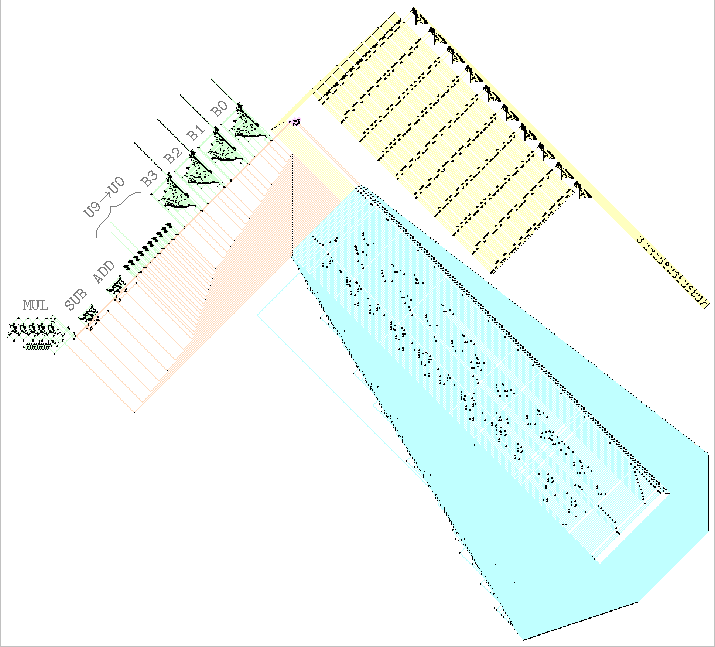
\includegraphics[width=\textwidth]{universal_computation/pi_calculator.pdf}}
	\caption{A $\pi$ calculator that uses a massive computer (highlighted in \bgbox{aquaback}{aqua}) based on the APGsembly code from Appendix~\ref{sec:appendix_apg}. It feeds into a component stack (highlighted in \bgbox{greenpastel}{green}) that contains every component that we have seen so far: $10$ sliding block registers, $4$ binary registers, and one each of the \texttt{ADD}, \texttt{SUB}, and \texttt{MUL} components. It also feeds into a character printer (highlighted in \bgbox{yellowback2}{yellow}) which, as of generation $8.3 \times 10^{13}$, has printed the first $14$ digits of $\pi$: $3.1415926535897$.}\label{fig:pi_calc}
\end{figure}


%%%%%%%%%%%%%%%%%%%%%%%%%%%%%%%%%%%%%%%%%%%%%%%%%%%%%%%%%%%%%%%%%%%%%%%%%
%%   SECTION: COMPUTING OTHER CONSTANTS
%%%%%%%%%%%%%%%%%%%%%%%%%%%%%%%%%%%%%%%%%%%%%%%%%%%%%%%%%%%%%%%%%%%%%%%%%
\subsection{Computing Other Constants}\label{sec:pi_calc_other}

This same algorithm that we used in our $\pi$ calculator can also be used to compute many other well-known mathematical constants. In particular, we can use that same method to construct patterns that print the digits of any number that can be represented by a series of the following form, where $a$, $b$, $p$, $q$, $r$, and $s$ are non-negative integers:\footnote{If $k = 0$ then the term $\frac{(p+q)(2p+q)\cdots(kp+q)}{(r+s)(2r+s)\cdots(kr+s)}$ is an ``empty product'', which equals $1$.}
\begin{align}\begin{split}\label{eq:generalized_pi_series}
		& \frac{a}{b}\sum_{k=0}^\infty \frac{(p+q)(2p+q)\cdots(kp+q)}{(r+s)(2r+s)\cdots(kr+s)} \\
		& \qquad\qquad = \frac{a}{b}\left(1 + \frac{p+q}{r+s}\left( 1 + \frac{2p+q}{2r+s}\left( 1 + \frac{3p+q}{3r+s}\left( \cdots \left( 1 + \frac{kp+q}{kr+s}\Big( \cdots \Big) \right)\right)\right)\right)\right).
\end{split}\end{align}
For example, the $\pi$ series~\eqref{eq:pi_series} arises in the case when $a = 2$, $b = 1$, $p = 1$, $q = 0$, $r = 2$, and $s = 1$.

All that changes in the algorithm and APGsembly code for computing a constant of this more general form, rather than $\pi$ itself, is that the $A_k$ matrices from Equation~\eqref{eq:Ak_matrices} should instead be defined by
\[
A_0 = \begin{bmatrix}
a & 0 \\ 0 & b
\end{bmatrix} \quad \text{and} \quad A_k = \begin{bmatrix}
kp+q & kr+s \\ 0 & kr+s
\end{bmatrix} \quad \text{for all} \quad k \geq 1.
\]
The computation of the $B_n$ matrices from the $A_k$s, as well as the remainder of the algorithm and pseudocode, stays the exact same.

To illustrate how to make this change to construct a calculator for a number other than $\pi$, consider the mathematical constant $e = 2.71828\ldots$, which makes frequent appearances in calculus and statistics. It has the well-known series representation
\begin{align}\label{eq:e_series}
	e = \sum_{k=0}^\infty \frac{1}{k!} = 1 + \left(1 + \frac{1}{2}\left(1 + \frac{1}{3}\left(1 + \frac{1}{4}\Big( \cdots \Big)\right)\right)\right),
\end{align}
corresponding to the values $a = 1$, $b = 1$, $p = 0$, $q = 1$, $r = 1$, and $s = 0$ in the general series~\eqref{eq:generalized_pi_series}. We can thus make the following two extremely minor changes to Pseudocode~\ref{alg:pseudocode_pi_calc} for computing $\pi$ to turn it into an algorithm for computing $e$:\smallskip

\begin{itemize}
	\item Replace line~2 with ``\texttt{set U0 = 1, B0 = 1, B2 = 1}''.\smallskip
	
	\item Replace line~8 with ``\texttt{set U1 = U1 + 1}''.\smallskip
\end{itemize}

More generally, to turn Pseudocode~\ref{alg:pseudocode_pi_calc} into pseudocode for computing a number via the series~\eqref{eq:generalized_pi_series}, we make the following changes based on the values of $a,b,p,q,r,$ and $s$:\smallskip

\begin{itemize}
	\item Replace line~2 with ``\texttt{set U0 = q, U1 = s, B0 = a, B2 = b}''.\smallskip
	
	\item Replace line~8 with ``\texttt{set U0 = U0 + p, U1 = U1 + r}''.\smallskip
\end{itemize}

Modifying the APGsembly code for the $\pi$ calculator from Appendix~\ref{sec:appendix_apg} is similarly straightforward. It can be turned into APGsembly for an $e$ calculator by just changing two or three lines of code: the \texttt{\#REGISTERS} line, the \texttt{ITER6;NZ} line, and optionally the \texttt{ITER7;ZZ} line (see Exercise~\ref{exer:universal_computation_e_calc}). Other constants like $\sqrt{2}$ can similarly be computed by making analogous minimal changes (see Exercise~\ref{exer:universal_computation_sqrt2_calc}).



%%%%%%%%%%%%%%%%%%%%%%%%%%%%%%%%%%%%%%%%%%%%%%%%%%%%%%%%%%%%%%%%%%%%%%%%%
%%   SECTION: 2D PRINTER
%%%%%%%%%%%%%%%%%%%%%%%%%%%%%%%%%%%%%%%%%%%%%%%%%%%%%%%%%%%%%%%%%%%%%%%%%
\section{A 2D Printer}\label{sec:2dprinter}

While the character printer that we introduced in Section~\ref{sec:decimal_printer} is quite flexible in that we can re-tool it to print any finite set of digits of our choosing, it is still limited by the fact that it can only print them linearly. The final component that we introduce, which we denote by \texttt{B2D}, solves this problem by being able to print an arbitrary pattern in an infinite 2D quadrant of the Life plane. Alternatively, this component can be thought of as a 2D generalization of the binary register from Section~\ref{sec:binary_register}: while that component kept track of an infinite 1D \emph{list} of bits, this one keeps track of an infinite 2D \emph{array} of bits.\footnote{This interpretation explains the abbreviation \texttt{B2D} for this component; it stands for ``binary 2-dimensional''.}

The way that this 2D printer works is almost the exact same as the binary register, but with two perpendicular sliding blocks to read and write the desired bits instead of just one. In particular, those sliding blocks are used to fire gliders at each other so as to synthesize or destroy boats that are laid out in a diagonal grid with a separation of $16$ full diagonals. These boats can either be interpreted as bits in some sort of computation (with a boat representing a \texttt{1} and an empty space representing a \texttt{0}), or they can be thought of as pixels in an image that can be viewed by zooming far out in Life simulation software.

In order to actually print those pixels (i.e., boats), the 2D printer can be called via APGsembly actions that are almost identical to those of the binary register, but with the minor extra complexity that we can increment and decrement the location of the 2D printer's read head \index{read head} in two different perpendicular directions. We say that the ``$x$'' direction of this grid is the diagonal running from southwest to northeast, and the ``$y$'' direction is the one running from southeast to northwest (so that the coordinate system for this printer is just the usual Cartesian coordinate system, but rotated counter-clockwise by $45$~degrees). Only points with non-negative $x$ and $y$ coordinates are accessible to the printer, so it can print on the top-central quadrant of the Life plane.

The APGsembly actions themselves are listed below, and since these are the last components and actions that we will make use of in this computational toolkit, this is a natural time to summarize them all. This summary is provided in Table~\ref{tab:universal_computation_components}.\smallskip

\begin{itemize}
	\item \texttt{INC B2DX} and \texttt{INC B2DY}, which move the pointer blocks of the read head one step farther away from the printer itself (northeast or northwest, respectively).\smallskip
	
	\item \texttt{TDEC B2DX} and \texttt{TDEC B2DY}, which move the pointer blocks to the previous location in the $x$ or $y$ direction (i.e., southwest or southeast), respectively, or keep them in the same place if they're already at the zero position. These actions also return either \texttt{Z} or \texttt{NZ}, depending on whether or not the $x$ or $y$ read head was already at the \texttt{0} location.\smallskip
	
	\item \texttt{READ B2D}, which sets the value of the bit at the current read head location to ``\texttt{0}''. This action returns either \texttt{Z} or \texttt{NZ}, depending on the original value of this bit.\smallskip
	
	\item \texttt{SET B2D}, which places a ``\texttt{1}'' bit at the current read head location.\footnote{Just like the binary register's \texttt{SET} action, this mechanism will self-destruct if a pixel is \texttt{SET} when a boat is already present at the current read head location.}\smallskip
\end{itemize}

\begin{table}[!phtb]
		\begin{tabular}{lll}
			\toprule
			Component & Actions & Functionality and return value \\\midrule
			\texttt{Un}: sliding block register & \texttt{INC Un} & increases the value of the register by \texttt{1}, no return value \\
			\hphantom{\texttt{Un}:} stores a non-negative & \cellcolor{gray!20}\texttt{TDEC Un} & \cellcolor{gray!20}returns \texttt{Z} if \texttt{Un = 0} and \texttt{NZ} otherwise, and \emph{then} \\
			\hphantom{\texttt{Un}:} integer in unary & \cellcolor{gray!20} & \cellcolor{gray!20}decreases the value of the register by \texttt{1} if \texttt{NZ} \\\midrule
			
			\texttt{Bn}: binary register & \texttt{INC Bn} & increases the position of the read head,\\
			\hphantom{\texttt{Bn}:} stores a non-negative & & no return value \\
			\hphantom{\texttt{Bn}:} integer in binary & \cellcolor{gray!20}\texttt{TDEC Bn} & \cellcolor{gray!20}returns \texttt{Z} if read head is at least significant bit and \\
			\hphantom{\texttt{Bn}:} & \cellcolor{gray!20} & \cellcolor{gray!20}\texttt{NZ} otherwise, and \emph{then} decreases position by \texttt{1} if \texttt{NZ} \\
			\hphantom{\texttt{Bn}:} & \texttt{READ Bn} & returns the bit (\texttt{Z = 0} or \texttt{NZ = 1}) at the read head, \\
			\hphantom{\texttt{Bn}:} & & and then sets it equal to \texttt{0} \\
			\hphantom{\texttt{Bn}:} & \cellcolor{gray!20}\texttt{SET Bn} & \cellcolor{gray!20}set the bit at the read head to \texttt{1}, no return value, \\
			\hphantom{\texttt{Bn}:} & \cellcolor{gray!20} & \cellcolor{gray!20}breaks if that bit already equals \texttt{1} \\\midrule
			
			\texttt{B2D}: 2D binary register & \texttt{INC B2DX} & increases the X position of the read head, \\
			\hphantom{\texttt{B2D}:} stores a 2D & & no return value \\
			\hphantom{\texttt{B2D}:} array of bits & \cellcolor{gray!20}\texttt{INC B2DY} & \cellcolor{gray!20}increases the Y position of the read head, \\
			\hphantom{\texttt{B2D}:} & \cellcolor{gray!20} & \cellcolor{gray!20}no return value \\
			\hphantom{\texttt{B2D}:} & \texttt{TDEC B2DX} & returns \texttt{Z} if X read head is at least significant bit and \\
			\hphantom{\texttt{B2D}:} & & \texttt{NZ} otherwise, and \emph{then} decreases X position by \texttt{1} if \texttt{NZ} \\
			\hphantom{\texttt{B2D}:} & \cellcolor{gray!20}\texttt{TDEC B2DY} & \cellcolor{gray!20}returns \texttt{Z} if Y read head is at least significant bit and \\
			\hphantom{\texttt{B2D}:} & \cellcolor{gray!20} & \cellcolor{gray!20}\texttt{NZ} otherwise, and \emph{then} decreases Y position by \texttt{1} if \texttt{NZ} \\
			
			\hphantom{\texttt{B2D}:} & \texttt{READ B2D} & returns the bit (\texttt{Z = 0} or \texttt{NZ = 1}) at the read head, \\
			\hphantom{\texttt{B2D}:} & & and then sets it equal to \texttt{0} \\
			\hphantom{\texttt{B2D}:} & \cellcolor{gray!20}\texttt{SET B2D} & \cellcolor{gray!20}set the bit at the read head to \texttt{1}, no return value, \\
			\hphantom{\texttt{B2D}:} & \cellcolor{gray!20} & \cellcolor{gray!20}breaks if that bit already equals \texttt{1} \\\midrule
			
			\texttt{ADD}: binary adder & \texttt{ADD A1} & helps us add one binary register to another one, \\
			& \texttt{ADD B0} & as in APGsembly~\ref{alg:apgsembly_binary_add_sub} \\
			& \texttt{ADD B1} & \\\midrule
			
			\texttt{SUB}: binary subtractor & \texttt{SUB A1} & helps us subtract one binary register from another one, \\
			& \texttt{SUB B0} & as in APGsembly~\ref{alg:apgsembly_binary_add_sub} \\
			& \texttt{SUB B1} & \\\midrule
			
			\texttt{MUL}: binary multiplier & \texttt{MUL 0} & helps us quickly multiply a binary register by \texttt{10}, \\
			& \texttt{MUL 1} & as in APGsembly~\ref{alg:apgsembly_mul_ten} \\\midrule
			\texttt{OUTPUT}: digit printer & \texttt{OUTPUT x} & prints \texttt{x} in a font made up of blocks, no return value,\\
			& & \texttt{x} must be one of \texttt{0}, \texttt{1}, \texttt{2}, \texttt{3}, \texttt{4}, \texttt{5}, \texttt{6}, \texttt{7}, \texttt{8}, \texttt{9}, or \texttt{.}\\\midrule
			
			\texttt{NOP}: no operation & \texttt{NOP} & returns \texttt{Z} and does nothing else\\\midrule
			
			\texttt{HALT\_OUT} & \texttt{HALT\_OUT} & halts the entire computation and emits a glider\\
			\bottomrule
		\end{tabular}
	\caption{A summary of the standard components that APGsembly can make use of and the actions that they can perform.}\label{tab:universal_computation_components}
\end{table}

The 2D printer is extremely large, so we do not display it here, but we will see it in the upcoming Figure~\ref{fig:osqrtlogt}. It is worth noting that this component is so slow and large that we actually have to use a slightly slower clock gun whenever it is present---one with period at least $2^{22}$ (instead of period $2^{20}$, like we have used until now). Indeed, if we use a clock gun that is too fast then a return value from another component might arrive back at the clock gun, starting the next clock tick, while the \texttt{B2D} component is still working on its previous action. If another action is then sent to the \texttt{B2D} component, it could lead to an unwanted collision.


%%%%%%%%%%%%%%%%%%%%%%%%%%%%%%%%%%%%%%%%%%%%%%%%%%%%%%%%%%%%%%%%%%%%%%%%%
%%   SECTION: KOCH SNOWFLAKE
%%%%%%%%%%%%%%%%%%%%%%%%%%%%%%%%%%%%%%%%%%%%%%%%%%%%%%%%%%%%%%%%%%%%%%%%%
\subsection{Printing a Fractal}\label{sec:koch_snowflake}\index{Koch snowflake}

To illustrate the flexibility of this 2D printer, we now demonstrate how it can be used to print a fractal. Slightly more accurately, we use it to print better and better approximations of a fractal, which of course is the best we could hope for---our printing capabilities are limited by the fact that we are working on the Life plane and thus must make our images out of pixels.

The way that we construct the fractal is to imagine walking along some path in the plane, printing a pixel after every step that we take. We always step a distance of $1$ in one of the eight orthogonal or diagonal directions (in the Moore neighborhood \index{Moore neighborhood} sense, so increasing both the $x$- and $y$-coordinates by $1$, for example, is a valid move). The path that we walk along is illustrated in Figure~\ref{fig:koch_algorithm}, and is determined as follows:\smallskip

\begin{figure}[!htb]
	\centering
	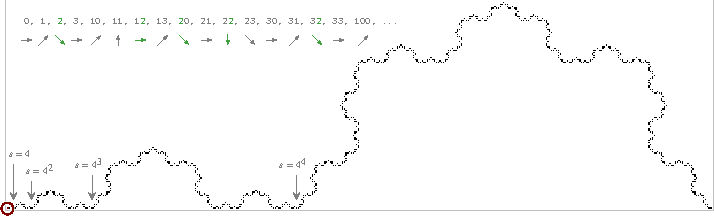
\includegraphics[width=\textwidth]{universal_computation/koch_algorithm.pdf}
	\caption{The (leftmost portion of the) image that results from starting at the bottom-left corner (circled in \bgbox{redback}{red}) and printing pixels according to a path-following procedure based on counting in base~$4$ (in the variable $s$). These bulbous shapes are better and better approximations of the top half of an 8-pointed version of the Koch snowflake fractal.}\label{fig:koch_algorithm}
\end{figure}


\clearpage%for layout reasons


\begin{itemize}
	\item[1)] Start at the coordinate $(x,y) = (0,0)$, facing right (toward the coordinate $(1,0)$).\smallskip
	
	\item[2)] Color in the pixel at the current location and then walk forward one step.\smallskip
	
	\item[3)] Let $s$ be the total number of steps that we have taken so far.\smallskip
	\begin{itemize}
		\item If $s$, when represented in base~$4$, has more ``\texttt{2}'' digits than $s-1$, turn clockwise by $90$ degrees.\smallskip
		
		\item Otherwise, turn counter-clockwise by $45$ degrees.\smallskip
	\end{itemize}
	
	\item[4)] Return to Step~(2).\smallskip
\end{itemize}

The above procedure results in a path that, on average, moves straight to the right. After all, every time we increase the total number of steps $s$ by one, exactly one digit rolls over to either \texttt{1}, \texttt{2}, or \texttt{3}. Two of those three possibilities result in our orientation rotating $45$ degrees counter-clockwise, and the other one of those three possibilities results in our orientation rotating $90$ degrees counter-clockwise, for a total average of no rotation at all.

The fractal-like behavior of this path comes from the repetitive nature of digit strings that are encountered when counting. Indeed, if we ever encounter a particular (base 4) string of digits in $s$ when counting, we will encounter that exact same string of digits infinitely many times later on too, as additional leading digits are added to $s$. The resulting fractal is the top half of an $8$-pointed version of a well-known fractal called the \textbf{Koch snowflake} (which is usually $6$-pointed).

APGsembly code that implements this algorithm is displayed in APGsembly~\ref{alg:apgsembly_koch}. Although it is somewhat long, it is reasonably straightforward and makes use of $5$ sliding block (unary) registers and one binary register to keep track of the following quantities:\smallskip

\begin{itemize}
	\item[\texttt{U0}:] stores the $x$-direction to move (\texttt{0} = none, \texttt{1} = right, \texttt{2} = left)
	
	\item[\texttt{U1}:] stores the $y$-direction to move (\texttt{0} = none, \texttt{1} = up, \texttt{2} = down)
	
	\item[\texttt{U2}:] a value that determines which of the 8 possible directions to move in at the next step (\texttt{0} = right, \texttt{1} = up-right, \texttt{2} = up, ..., \texttt{7} = down-right)---\texttt{U0} and \texttt{U1} are computed based on this
	
	\item[\texttt{U3}:] a temporary helper register
	
	\item[\texttt{U4}:] the amount to add to \texttt{U2} after we encounter an extra ``\texttt{2}'' when counting in base~$4$ (stays constant at \texttt{6}, corresponding to a clockwise turn by $90$ degrees)
	
	\item[\texttt{U5}:] how much to mod \texttt{U2} by after adding to it (stays constant at \texttt{8})\smallskip
	
	\item[\texttt{B0}:] keeps track of the number of steps that we have taken in base~$4$ ($= s$)\smallskip
\end{itemize}

\begin{apgsembly}
	\centering
	\begin{minipage}[t]{.49\textwidth}
		\begin{algorithmic}\tiny
			\State \verb|#COMPONENTS U0-5,B0,B2D,NOP|
			\State \verb|#REGISTERS {'U4':6, 'U5':8}|
			\State \verb|# State   Input   Next state   Actions|
			\State \verb|# ---------------------------------------|
			\State \verb|INITIAL;  ZZ;     DIR0;        TDEC U2|
			\State
			\State \verb|# Update U0 and U1, based on U2, so that we walk in the correct|
			\State \verb|# direction. Also set U3 = U2 and then U2 = 0.|
			\State \verb|DIR0;     Z;      RESETU2;     TDEC U3, INC U0|
			\State \verb|DIR0;     NZ;     DIR1;        TDEC U2, INC U3|
			\State \verb|DIR1;     Z;      RESETU2;     TDEC U3, INC U0, INC U1|
			\State \verb|DIR1;     NZ;     DIR2;        TDEC U2, INC U3|
			\State \verb|DIR2;     Z;      RESETU2;     TDEC U3, INC U1|
			\State \verb|DIR2;     NZ;     DIR3;        TDEC U2, INC U3|
			\State \verb|DIR3;     Z;      DIRX;        INC U0, INC U1, NOP|
			\State \verb|DIR3;     NZ;     DIR4;        TDEC U2, INC U3|
			\State \verb|DIR4;     Z;      DIRX;        INC U0, NOP|
			\State \verb|DIR4;     NZ;     DIR5;        TDEC U2, INC U3|
			\State \verb|DIR5;     Z;      DIRXY;       INC U0, INC U1, NOP|
			\State \verb|DIR5;     NZ;     DIR6;        TDEC U2, INC U3|
			\State \verb|DIR6;     Z;      DIRY;        INC U1, NOP|
			\State \verb|DIR6;     NZ;     DIRY;        INC U0, INC U1, INC U3, NOP|
			\State \verb|DIRX;     ZZ;     RESETU2;     TDEC U3, INC U0|
			\State \verb|DIRY;     ZZ;     RESETU2;     TDEC U3, INC U1|
			\State \verb|DIRXY;    ZZ;     RESETU2;     TDEC U3, INC U0, INC U1|
			\State
			\State \verb|# Restore U2 from value in temporary register U3, and then draw|
			\State \verb|# the pixel (boat) at the current bit.|
			\State \verb|RESETU2;  Z;      DRAWX1;      TDEC U0, SET B2D|
			\State \verb|RESETU2;  NZ;     RESETU2;     TDEC U3, INC U2|
			\State
			\State \verb|# Update the B2D read head location based on U0 and U1.|
			\State \verb|DRAWX1;   Z;      DRAWY1;      TDEC U1|
			\State \verb|DRAWX1;   NZ;     DRAWX2;      TDEC U0|
			\State \verb|DRAWX2;   Z;      DRAWY1;      TDEC U1, INC B2DX|
			\State \verb|DRAWX2;   NZ;     DRAWX3;      TDEC B2DX|
			\State \verb|DRAWX3;   *;      DRAWY1;      TDEC U1|
			\State \verb|DRAWY1;   Z;      RESETB0;     TDEC B0|
			\State \verb|DRAWY1;   NZ;     DRAWY2;      TDEC U1|
			\State \verb|DRAWY2;   Z;      RESETB0;     TDEC B0, INC B2DY|
			\State \verb|DRAWY2;   NZ;     DRAWY3;      TDEC B2DY|
			\State \verb|DRAWY3;   *;      RESETB0;     TDEC B0|
		\end{algorithmic}
	\end{minipage}\hfill{\color{gray}\vline}\hfill
	\begin{minipage}[t]{.49\textwidth}
		\begin{algorithmic}\tiny
			\State \verb|# Move B0 read head to least significant bit.|
			\State \verb|RESETB0;  Z;      INCB0A;      READ B0|
			\State \verb|RESETB0;  NZ;     RESETB0;     TDEC B0|
			\State
			\State \verb|# Add 1 to B0. If we introduce a new "2" in its base-4|
			\State \verb|# representation, go to INCU2A, otherwise add 1 to U2.|
			\State \verb|INCB0A;   Z;      INCB0B;      SET B0, NOP|
			\State \verb|INCB0A;   NZ;     INCB0E;      INC B0, NOP|
			\State \verb|INCB0B;   ZZ;     INCB0C;      INC B0, NOP|
			\State \verb|INCB0C;   ZZ;     INCB0D;      READ B0|
			\State \verb|INCB0D;   Z;      MOD8A;       TDEC U5, INC U2|
			\State \verb|INCB0D;   NZ;     MOD8A;       TDEC U5, INC U2, SET B0|
			\State \verb|INCB0E;   ZZ;     INCB0F;      READ B0|
			\State \verb|INCB0F;   Z;      INCU2A;      TDEC U4, SET B0|
			\State \verb|INCB0F;   NZ;     RESETB0;     INC B0, NOP|
			\State
			\State \verb|# Add U4 (= 6) to U2 with the help of U0, without clearing U4.|
			\State \verb|INCU2A;   Z;      INCU2B;      TDEC U0|
			\State \verb|INCU2A;   NZ;     INCU2A;      TDEC U4, INC U0, INC U2|
			\State \verb|INCU2B;   Z;      MOD8A;       TDEC U5|
			\State \verb|INCU2B;   NZ;     INCU2B;      TDEC U0, INC U4|
			\State
			\State \verb|# Set U2 = U2 mod (U5 = 8), with the help of U0 and U1.|
			\State \verb|MOD8A;    Z;      RESET3;      TDEC U1|
			\State \verb|MOD8A;    NZ;     MOD8B;       TDEC U2, INC U0|
			\State \verb|MOD8B;    Z;      RESET1;      TDEC U0|
			\State \verb|MOD8B;    NZ;     MOD8A;       TDEC U5, INC U1|
			\State
			\State \verb|# Reset registers and restart.|
			\State \verb|RESET1;   *;      RESET2;      TDEC U0|
			\State \verb|RESET2;   Z;      RESET3;      TDEC U1, INC U5|
			\State \verb|RESET2;   NZ;     RESET2;      TDEC U0, INC U2|
			\State \verb|RESET3;   Z;      RESET4;      TDEC U0|
			\State \verb|RESET3;   NZ;     RESET3;      TDEC U1, INC U5|
			\State \verb|RESET4;   Z;      DIR0;        TDEC U2|
			\State \verb|RESET4;   NZ;     RESET4;      TDEC U0|
		\end{algorithmic}
	\end{minipage}
	\caption{APGsembly code for the $8$-pointed Koch snowflake printer.}\label{alg:apgsembly_koch}
\end{apgsembly}

Since the 2D printer component prints on a diagonal grid, the Life pattern that implements this APGsembly code\footnote{Originally constructed by Michael Simkin in 2019.} prints the image from Figure~\ref{fig:koch_algorithm} rotated counter-clockwise by $45$ degrees. We leave the actual compilation of this Life pattern to Exercise~\ref{exer:universal_computation_b2d_why_far}.


%%%%%%%%%%%%%%%%%%%%%%%%%%%%%%%%%%%%%%%%%%%%%%%%%%%%%%%%%%%%%%%%%%%%%%%%%
%%   SECTION: OSQRTLOGT
%%%%%%%%%%%%%%%%%%%%%%%%%%%%%%%%%%%%%%%%%%%%%%%%%%%%%%%%%%%%%%%%%%%%%%%%%
\subsection{An Extremely Slowly Growing Pattern}\label{sec:Osqrtlogt}

We now return to the problem of creating a pattern with a very slowly growing bounding box, which we first considered via a binary ruler in Section~\ref{sec:binary_ruler}. In an $n \times n$ bounding box, there are $n^2$ different cells that can each be in one of $2$ states, for a total of $2^{n^2}$ possible different patterns. It follows that if a pattern exhibits infinite growth then it cannot stay within an $n \times n$ bounding box past generation $t = 2^{n^2}$, since after that point in time its phases would necessarily start repeating.

If we flip this argument around and solve for $n$ in terms of $t$, we see that in generation~$t$, the bounding box of an infinitely growing pattern can be no smaller than $\sqrt{\log_2(t)} \times \sqrt{\log_2(t)}$.\footnote{This contrasts with our results of Section~\ref{sec:recursive_filter}: even though there is no slowest \emph{population} growth rate, there is a slowest \emph{bounding box} growth rate.} We now construct a pattern that attains this minimum possible bounding box growth rate, at least asymptotically---its diameter in generation~$t$ is $\Theta(\sqrt{\log(t)})$.

The basic idea behind this slowly growing pattern is the same as it was for the binary ruler from Section~\ref{sec:binary_ruler}, which had diameter $\Theta(\log(t))$. We count in binary, except instead of placing the bits of the resulting number in a single 1D row via a binary register, we arrange them in a 2D triangular array via a 2D printer. In particular, we place the least significant bit of the number in one row, the next $2$ least significant bits in the next row, the next $3$ least significant bits in the next row, and so on. The APGsembly code that performs this task is presented in APGsembly~\ref{alg:apgsembly_slow_growth}.

\begin{apgsembly}
	\begin{algorithmic}\small
		\State \verb|#COMPONENTS B2D,NOP,U0-2|
		\State \verb|#REGISTERS {}|
		\State \verb|# State    Input    Next state    Actions|
		\State \verb|# ---------------------------------------|
		\State \verb|INITIAL;   ZZ;      CHECK;        READ B2D|
		\State
		\State \verb|## Determine whether the current bit equals 0 or 1.|
		\State \verb|# If it equals 0, set it to 1 and go to the least significant bit.|
		\State \verb|# If it equals 1, set it to 0 and go to the next most significant bit.|
		\State \verb|CHECK;     Z;       LSB1;         SET B2D, NOP|
		\State \verb|CHECK;     NZ;      NSB1;         TDEC U0|
		\State
		\State \verb|## The LSB states move the B2D read head to (0,0) and set U0 = U1 = 0.|
		%		\State \verb|# Set B2D read head X coordinate to 0 and then jump to Y coordinate code.|
		\State \verb|LSB1;      ZZ;      LSB2;         TDEC B2DX|
		\State \verb|LSB2;      Z;       LSB3;         TDEC B2DY|
		\State \verb|LSB2;      NZ;      LSB2;         TDEC B2DX|
		%		\State
		%		\State \verb|# Set B2D read head Y coordinate to 0 and then jump to U0 code.|
		\State \verb|LSB3;      Z;       LSB4;         TDEC U0|
		\State \verb|LSB3;      NZ;      LSB3;         TDEC B2DY|
		%		\State
		%		\State \verb|# Set U0 = 0 and then jump to U1 code.|
		\State \verb|LSB4;      Z;       LSB5;         TDEC U1|
		\State \verb|LSB4;      NZ;      LSB4;         TDEC U0|
		%		\State
		%		\State \verb|# Set U1 = 0 and then read the current bit (the bit at (0,0)).|
		\State \verb|LSB5;      Z;       CHECK;        READ B2D|
		\State \verb|LSB5;      NZ;      LSB5;         TDEC U1|
		\State
		\State \verb|## The NSB states move the B2D read head to the next most significant bit.|
		\State \verb|# If U0 = 0 then we are at the end of the current X row, so start the next one.|
		\State \verb|# If U0 > 0 then go to the next position in this X row and read the bit.|
		\State \verb|NSB1;      Z;       NSB3;         TDEC B2DX|
		\State \verb|NSB1;      NZ;      NSB2;         INC B2DX, NOP|
		\State \verb|NSB2;      ZZ;      CHECK;        READ B2D|
		\State
		\State \verb|# When going to the next X row, increase U1 (the length of the current X row).|
		\State \verb|NSB3;      Z;       NSB4;         INC B2DY, INC U1, NOP|
		\State \verb|NSB3;      NZ;      NSB3;         TDEC B2DX|
		\State
		\State \verb|# Copy U1 into U0, with the help of U2. Then read the current bit.|
		\State \verb|NSB4;      ZZ;      NSB5;         TDEC U1|
		\State \verb|NSB5;      Z;       NSB6;         TDEC U2|
		\State \verb|NSB5;      NZ;      NSB5;         TDEC U1, INC U2|
		\State \verb|NSB6;      Z;       CHECK;        READ B2D|
		\State \verb|NSB6;      NZ;      NSB6;         TDEC U2, INC U0, INC U1|
	\end{algorithmic}
	\caption{APGsembly code for a pattern whose diameter (i.e., longest bounding box side length) in generation~$t$ is $\Theta(\sqrt{\log(t)})$---the smallest unbounded diametric growth rate possible.}\label{alg:apgsembly_slow_growth}
\end{apgsembly}

This APGsembly code is quite a bit longer, but not much more complicated, than APGsembly~\ref{alg:apgsembly_binary_ruler} for the binary ruler. The only extra complexity in this code is that we need some unary registers to help us keep track of how many bits in total we should print in the current row, and how many bits are left before we reach the end of the current row. In particular, it makes use of three sliding block registers as follows:\smallskip

\begin{itemize}
	\item[\texttt{U0}:] the number of bits left to print before reaching the end of the current row
	
	\item[\texttt{U1}:] the total number of bits to print in the current row
	
	\item[\texttt{U2}:] a helper register used to copy \texttt{U1} into \texttt{U0} when we start a new row\smallskip
\end{itemize}

The pattern that results from compiling this APGsembly code is displayed in Figure~\ref{fig:osqrtlogt}. To give an idea of how slowly the diameter of this pattern grows, note in the $7.5 \times 10^{11}$ generations after printing its first bit (i.e., boat), its computer goes through roughly $44{\thousep}700$ clock ticks and the pattern's bounding box increases in size by only $64$ cells in one direction and $96$ cells in the other.\footnote{The boats that the 2d printer prints are offset from each other by $16$ full diagonals.} We could slow down this pattern even more by decreasing the speed of its clock gun, but that would not change the asymptotic growth rate of its diameter.

\begin{figure}[!htb]
	\centering
	\embedlink{osqrtlogt}{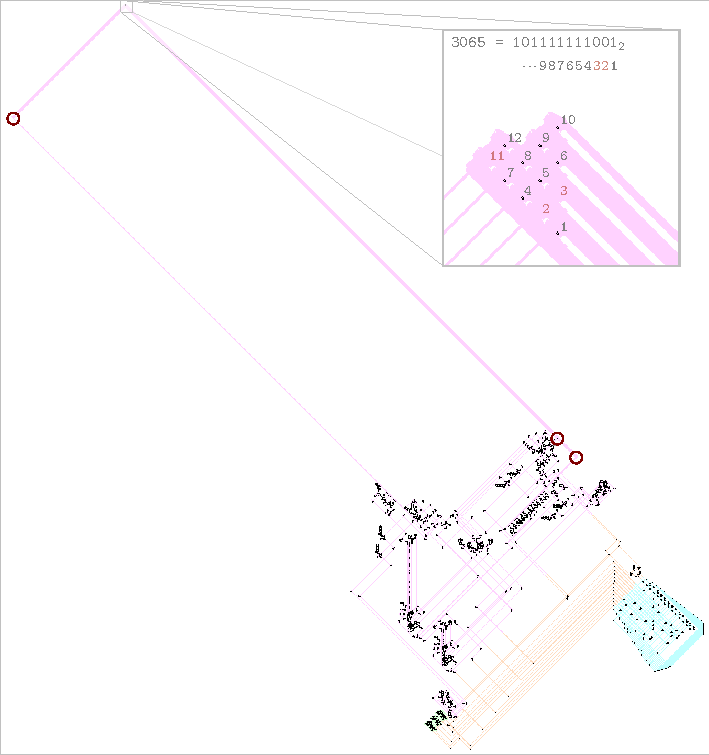
\includegraphics[width=\textwidth]{universal_computation/osqrtlogt.pdf}}
	\caption{A pattern with minimal asymptotic diametric growth rate $\Theta(\sqrt{\log(t)})$, compiled from APGsembly~\ref{alg:apgsembly_slow_growth}. The computer at the bottom-right, highlighted in \bgbox{aquaback}{aqua}, feeds into three sliding block registers (highlighted in \bgbox{greenpastel}{green}) and a 2D printer (highlighted in \bgbox{magentaback}{magenta}). The 2D printer makes use of three sliding blocks (circled in \bgbox{redback}{red}) to create and read a 2D array of boats at the top that can in principle extend arbitrarily far to the northwest and northeast. This particular computer counts in binary and instructs the 2D printer to arrange the bits of the current number as boats in a triangle (which gets larger as the number of bits increases). After $7.5 \times 10^{11}$ generations, it has counted to $3065 = 101111111001_2$.}\label{fig:osqrtlogt}
\end{figure}


%%%%%%%%%%%%%%%%%%%%%%%%%%%%%%%%
\section{Notes and Historical Remarks}\label{sec:universal_computation_history}
%%%%%%%%%%%%%%%%%%%%%%%%%%%%%%%%

Conway's and Gosper's groups showed in the early 1970s that it was theoretically possible to assemble a Life pattern to complete any computational task that a standard programmable computer could accomplish \cite{Wain74,BCG82}. However, it wasn't until almost three decades later that Life technology advanced far enough to allow for universal computer patterns that were small enough to be simulated on a desktop computer.

Paul Rendell developed the first such device in April 2000 \cite{RenBook}---a Turing machine based on period~30 circuitry (stable circuitry was not nearly as well-developed at the time). He then extended this to a \emph{universal} Turing machine (i.e., a device capable of emulating any Turing machine) in February 2010. While these devices are computationally universal, and their input and output are reasonably straightforward to interpret, Turing machines themselves are rather abstract. For example, programming this device to compute (let alone display) the digits of $\pi$ would be a monumental task.

Paul Chapman constructed the next universal computer in 2002---a register machine that, at a high level, functions much like the universal computation toolkit that we introduced in this chapter.\footnote{See \httpurl{www.igblan.free-online.co.uk/igblan/ca/} for pattern files and a description of this machine.} Indeed, it made use of sliding blocks to build unary registers (just like we did), and switched between different states by virtue of actions to those unary registers returning zero or non-zero values. However, it used lightweight spaceships to transmit information instead of gliders, it made use of period~30 circuitry instead of stable circuitry, and it did not have any of the other components (e.g., binary registers or character printers) that we introduced.

The next universal computation toolkit to be developed was the one that we explored in this chapter, which was completed by Adam P.~Goucher in 2010 \cite{Gou10}. Finally, Nicolas Loizeau created an 8-bit programmable computer in 2016.\footnote{See \httpsurl{conwaylife.com/wiki/8-bit_programmable_computer} for download links and usage instructions.} While it is less versatile than the toolkit from this chapter (e.g., it cannot compute quantities larger than $2^8-1 = 255$), it is significantly simpler to program. For example, just $8$ relatively easy-to-understand lines of code suffice to program it to compute the sequence of Fibonacci numbers (up to the term $233$, which is the largest one it can handle), whereas a few dozen lines of somewhat more complicated APGsembly code would be required to compute that sequence (see Exercise~\ref{exer:universal_computation_print_fibonacci}).\index{Fibonacci number}

The original $\pi$ calculator that Adam P.~Goucher built in February~2010 had a bounding box that was roughly $12$ times as large as the one that we displayed in Figure~\ref{fig:pi_calc}, since many of the small components that we used (like Snarks and syringes) were not available at that time. However, the actual functionality of our calculator is almost identical to that of the original one, as is the speed at which it runs.

About one week prior to building his $\pi$ calculator, Goucher built a similar calculator for the mathematical constant $\varphi = (1+\sqrt{5})/2 = 1.61803\ldots$. While the techniques of Section~\ref{sec:pi_calc_other} are general enough to build a $\varphi$ calculator, the original one used a much simpler algorithm that caused it to run significantly faster---it could compute the first $n$ digits of $\varphi$ in $\Theta(n^3)$ generations, whereas the $\pi$~calculator requires $\Theta(n^6)$ generations for the same task.
% Explanation of pi calculator runtime:
% Binary registers are allocated with Theta(n^2) bits of memory in pi calc
% Multiplication steps like U0 * B0 thus require Theta(n^3) operations (Theta(n) additions, each of which requires Theta(n^2) bit operations)
% Digit extraction also requires Theta(n^3) operations, since we do no more than 10n subtractions to extract the n-th bit. Each of those subtractions again requires Theta(n^2) bit operations).
% Altogether, Theta(n^3) operations (i.e., states) to compute n-th digit, so Theta(n^4) operations to compute ALL first n digits. However, once n gets big enough, it takes more than 1 clock tick to perform a bit operation. This pushes us up to Theta(n^6).


% TODO:  Exercise: 1) In APGsembly 1.1, if the INITIAL state were removed, what line of code would the program have to start on to make its behavior the same as before?  (Answer: it would work to start execution on the ID3 NZ line.) 2) Why can't we remove the INITIAL state and produce re-ordered APGsembly code that performs the same algorithm with one less state?  (Answer: to start the program we have to run a command to produce an initial return value.  We could reorder the states to make ID3 the initial state, but then we'd also have to start the program with an initial ``NZ'' return value.  We could certainly set up the Life pattern to work that way, but it's traditional to not assume a specific return value until we run an INITIAL instruction to generate it.)

% TODO?: Exercise -- Why/how do ADD/SUB differ? How do they store a memory bit?
% TODO?: Exercise -- Copy binary register into another one?
% TODO: Exercise to compile the "store 139" APGsembly into a real pattern.

% TODO: Exercise to create APGsembly that prints an elementary cellular automaton (https://www.conwaylife.com/forums/viewtopic.php?f=2&t=4196&hilit=textbook&start=75#p104465)
% Exercise todo: identify the 6 inputs to the 2d printer from left-to-right.
% Exercise explaining why o(n^6)?


%%%%%%%%%%%%%%%%%%%%%%%%%%%%%%%%%
\section*{Exercises \hfill \normalfont\textsf{\small solutions to starred exercises on \hyperlink{solutions_universal_computation}{page \pageref{solutions_universal_computation}}}}
\label{sec:solutions_universal_computation}
\addcontentsline{toc}{section}{Exercises}
\vspace*{-0.4cm}\hrulefill\vspace*{-0.3cm}\footnotesize\begin{multicols}{2}\vspace*{-0.4cm}\raggedcolumns\interlinepenalty=10000
	\setlength{\parskip}{0pt}\ifdefined\FORPRINTING\colorlet{ocre}{black}\else%
\fi
	%%%%%%%%%%%%%%%%%%%%%%%%%%%%%%%%%
	
	
	\begin{problem}\label{exer:universal_computation_apgsembly_le_ge_eq} \probdiff{2}
		Add some additional lines of APGsembly code to APGsembly~\ref{alg:apgsembly_test_leq_or_ge} so as to make it have $3$ possible outputs instead of just $2$: one corresponding to \texttt{U0 < U1}, one to \texttt{U1 < U0}, and one to \texttt{U0 = U1}.
	\end{problem}
	
	
	\mfilbreak
	
	
	\begin{problem}\label{exer:universal_computation_apgsembly_leq_ge_reset} \probdiff{2}
		Modify APGsembly~\ref{alg:apgsembly_test_leq_or_ge}, with the help of additional registers, so that the \texttt{U0} and \texttt{U1} registers return to their original values at the end of the program. How many additional registers do you need to accomplish this task?
	\end{problem}
	% SOLUTION: four additional registers would make it easy---DEC U0 and U1 while INCing U2 and U3, then DEC U2 and U3 while INCing U4 and U5 and re-INCing U0 and U1, then leave U0 and U1 untouched after that and revise the above code to operate on U4 and U5. It can be done with only two additional registers, or even only one, with increasingly unreasonable amounts of extra code.
	
	
	\mfilbreak
	
	
	\begin{problem}\label{exer:universal_computation_mult_preserve_r0} \probdiff{2}
		Modify APGsembly~\ref{apg:mult_unary_reg} for multiplying two sliding block registers so as to complete the same computation without erasing the value of \texttt{U0}.
		
		\noindent [Hint: Add another temporary register.]
	\end{problem}
	
	
	\mfilbreak
	
	
	\begin{problem}\label{exer:division_by_subtraction} \probdiff{3}
		In this exercise, we implement the division-by-subtraction algorithm that was described at the end of Section~\ref{sec:multiply_two_registers}.\smallskip
		
		\begin{enumerate}[label=\bf\color{ocre}(\alph*)]
			\item Write pseudocode (similar in style to the pseudocode on the left of APGsembly~\ref{apg:mult_unary_reg}) that computes and stores the integer part of \texttt{U0 / U1} in \texttt{U2} and the remainder of that division in \texttt{U3}. You may use as many temporary registers as you like.
			
			\item Write APGsembly code that implements your pseudocode from part~(a).
			
			\item What happens in your code if \texttt{U1 = 0} and you try to divide by it? Modify your code, if necessary, so that it halts and provides some sort of error code in this case (e.g., maybe it could set some designated ``error register'' \texttt{U4} to \texttt{1}).
			
			\item Use the APGsembly compiler that is linked from \httpsurl{conwaylife.com/wiki/APGsembly} to compile a Life pattern that implements your APGsembly code from part~(b).
		\end{enumerate}
	\end{problem}


	\mfilbreak
	
	
	\begin{problem}\label{exer:describe_binary_register} \probdiff{2}
		Describe how the \texttt{READ} and \texttt{SET} actions of the binary register from Figure~\ref{fig:binary_register} are implemented. For example, what glider salvos implement these operations, and how are those salvos constructed?
	\end{problem}
	
	
	\mfilbreak
	
	
	\begin{problem}\label{exer:universal_computation_apgsembly_set_binary_value} \probdiff{1}
		Write APGsembly code that stores the value $241$ in a binary register \texttt{B0} (using \texttt{INC} and \texttt{SET} actions as in APGsembly~\ref{apg:store_139}, not via the \texttt{\#REGISTERS} header).
	\end{problem}
	
	
	\mfilbreak
	
	
	\begin{problem}\label{exer:universal_computation_apgsembly_multiply_binary} \probdiff{3}
		Suppose that \texttt{U0} and \texttt{B0} are a sliding block and binary register, respectively, storing some values. Write APGsembly code that computes \texttt{U0 * B0} and stores it in \texttt{B0}.
	\end{problem}
	
	
	\mfilbreak
	
	
	\begin{problem}\label{exer:universal_computation_apgsembly_exponentiate}
		In this exercise, suppose that \texttt{U0} is a sliding block register whose value has already been set.\smallskip
		
		\begin{enumerate}[label=\bf\color{ocre}(\alph*)]
			\item \probdiff{2} Write APGsembly code that stores the value $2^{\texttt{U0}}$ in the binary register \texttt{B0}.
			% Solution: Just do it bitwise. Easy.
			
			\item \probdiff{3} Write APGsembly code that stores the value $10^{\texttt{U0}}$ in the binary register \texttt{B0}.
			% Solution: Use MUL 10 code U0 times. Easy-ish.
			
			\item \probdiff{4} Write APGsembly code that stores the value $3^{\texttt{U0}}$ in the binary register \texttt{B0}.
			% Solution: Repeat the multiplication code from Exercise~\ref{exer:universal_computation_apgsembly_multiply_binary}. A bit harder.
		\end{enumerate}
	\end{problem}
	
	
	\mfilbreak
	
	
	\begin{problem}\label{exer:universal_computation_apgsembly_binary_compare} \probdiff{4}
		Write APGsembly code that determines which of two binary registers \texttt{B0} and \texttt{B1} is storing a larger value (i.e., code that outputs different results depending on whether \texttt{B0 <= B1} or \texttt{B1 < B0}, analogous to APGsembly~\ref{alg:apgsembly_test_leq_or_ge} for unary registers).
	\end{problem}
	% SOLUTION: can be extracted from pi calc
	
	
	\mfilbreak
	
	
	\begin{problemstar}\label{exer:binary_ruler_when_big} \probdiff{3}
		The binary ruler displayed in Figure~\ref{fig:binary_ruler} has a bounding box that is roughly $3{\thousep}600 \times 3{\thousep}100$ cells. At approximately what generation will the size of its bounding box first exceed $10{\thousep}000 \times 10{\thousep}000$? [Hint: Do not try to run it long enough to find out---do a calculation instead.]
	\end{problemstar}


	\mfilbreak
	
	
	\begin{problem}\label{exer:osqrtlogt_ruler_when_big} \probdiff{3}
		The extremely slowly growing pattern displayed in Figure~\ref{fig:osqrtlogt} has a bounding box that is roughly $24{\thousep}300 \times 26{\thousep}500$ cells. At approximately what generation will the size of its bounding box first exceed $30{\thousep}000 \times 30{\thousep}000$?
	\end{problem}


	\mfilbreak
	
	
	\begin{problem}\label{exer:binary_ruler_label} \probdiff{2}
		Label the northeast--southwest lines in the computer portion of the binary ruler from Figure~\ref{fig:binary_ruler} (like we labelled those lines in the multiplication computer of Figure~\ref{fig:mult_computer}). Which substate do each of these lines correspond to in APGsembly~\ref{alg:apgsembly_binary_ruler}?
	\end{problem}


	\mfilbreak
	
	
	\begin{problem}\label{exer:update_add_sub_mult} \probdiff{5}
		The \texttt{ADD}, \texttt{SUB}, and \texttt{MUL} components of Figures~\ref{fig:add_component}--\ref{fig:mul_component} were designed over a decade ago, and could be made much smaller via modern components like Snarks and syringes.\smallskip
		
		\begin{enumerate}[label=\bf\color{ocre}(\alph*)]
			\item Rebuild the \texttt{ADD} component, without sacrificing or changing any of its high-level functionality, so that it fits within an $800 \times 800$ bounding box.
			
			\item Rebuild the \texttt{SUB} component so that it fits within an $800 \times 800$ bounding box.
			
			\item Rebuild the \texttt{MUL} component so that it fits within a $1{\thousep}500 \times 1{\thousep}500$ bounding box.
		\end{enumerate}
	\end{problem}


	\mfilbreak
	
	
	\begin{problem}\label{exer:row_printer_six_not_seven} \probdiff{2}
		In the green pixel-printing portion of the row printer from Figure~\ref{fig:row_printer}, there are only 6 Herschel edge-shooters, yet they produce all 7 of the pixel-printing gliders from Figure~\ref{fig:char_printer_place_pixel}. Explain where the extra glider comes from.
	\end{problem}


	\mfilbreak
	
	
	\begin{problemstar}\label{exer:pi_calc_distant_merge} \probdiff{2}
		In the $\pi$ calculator of Figure~\ref{fig:pi_calc}, one of the computer's merge circuits (i.e., transparent reflectors) is significantly farther west than any of the others. Why? Which substate (i.e., line of APGsembly code from Appendix~\ref{sec:appendix_apg}) does this correspond to?
	\end{problemstar}
	
	
	\mfilbreak
	
	
	\begin{problemstar}\label{exer:universal_computation_derive_pi_series} \probdiff{4}
		In this exercise, we explore where the series~\eqref{eq:pi_series} for $\pi$ comes from.\smallskip
		
		\begin{enumerate}[label=\bf\color{ocre}(\alph*)]
			\item Explain why $\pi = 4 - 4/3 + 4/5 - 4/7 + 4/9 - \cdots$.
			
			[Hint: We did this already in Section~\ref{sec:periodic_circuits_notes}.]
			
			\item Manipulate the series from part~(a) to show that
			\[
			\pi = 2 + \left(\frac{4}{1\cdot 3} - \frac{4}{3\cdot 5} + \frac{4}{5\cdot 7} - \frac{4}{7\cdot 9} + \frac{4}{9\cdot 11} - \cdots\right).
			\]
			
			[Hint: Write each term $4/(2k+1)$ as $2/(2k+1) + 2/(2k+1)$ and regroup parentheses.]
			
			\item Use the same method on the parenthesized terms from part~(b) to rewrite that series as
			\[
			\pi = 2 + \frac{2}{3} + \left(\frac{8}{1\cdot 3 \cdot 5} - \frac{8}{3\cdot 5 \cdot 7} + \frac{8}{5\cdot 7 \cdot 9} - \cdots\right).
			\]
			
			\item Repeat this method over and over again to rewrite this series as
			\[
			\pi = 2\left(1 + \frac{1!}{3} + \frac{2!}{3\cdot 5} + \frac{3!}{3\cdot 5 \cdot 7} + \frac{4!}{3 \cdot 5 \cdot 7 \cdot 9} + \cdots\right).
			\]
			
			\item Finally, repeatedly factor the series from part~(d) to obtain the series~\eqref{eq:pi_series}.
			
			[Side note: This method of converting an alternating series into one with non-negative terms is called the \textbf{Euler transform}.]
		\end{enumerate}
	\end{problemstar}


	\mfilbreak
	
	
	\begin{problemstar}\label{exer:pi_calc_prove_correct} \probdiff{5}
		We claimed in the text that if the matrix $A_k$ is as defined in Equation~\eqref{eq:Ak_matrices}, $B_n = A_0A_1A_2\cdots A_n$, $q_n$ is the top-right entry of $B_n$, and $r_n$ is the bottom-right entry of $B_n$, then
		\[
			\frac{q_n}{r_n} = 2\left(1 + \frac{1}{3}\left( 1 + \frac{2}{5}\left( 1 + \frac{3}{7}\left( \cdots \left( 1 + \frac{n-1}{2n-1}\right)\right)\right)\right)\right),
		\]
		so the entries of $B_n$ can be used to approximate $\pi$. Prove this formula. [Hint: You can find fairly explicit formulas for the entries of $B_n$.]
	\end{problemstar}
	
	
	\mfilbreak
	
	
	\begin{problemstar}\label{exer:universal_computation_e_calc} \probdiff{3}
		Modify just $2$ or $3$ lines of the APGsembly code from Appendix~\ref{sec:appendix_apg} to turn the $\pi$ calculator into an $e$ calculator.
		
		\noindent [Hint: We described the changes that need to be made in Section~\ref{sec:pi_calc_other}.]
	\end{problemstar}
	
	
	\mfilbreak
	
	
	\begin{problem}\label{exer:universal_computation_sqrt2_calc}
		In this exercise, we use the following series to tweak the $\pi$ calculator to instead compute
		\begin{align*}
			\sqrt{2} = \sum_{k=0}^\infty \frac{(2k+1)!}{2^{3k+1}(k!)^2 } = \frac{1}{2} +\frac{3}{8} + \frac{15}{64} + \frac{35}{256} + \frac{315}{4096} + \cdots.
		\end{align*}
		
		\begin{enumerate}[label=\bf\color{ocre}(\alph*)]
			\item \probdiff{2} The above series representation of $\sqrt{2}$ can be put in the general form~\eqref{eq:generalized_pi_series}. What are the values of $a$, $b$, $p$, $q$, $r$, and $s$?
			% SOLUTION: a = 1, b = 2, p = 2, q = 1, r = 4, s = 0
			
			\item \probdiff{3} Change just a few lines of the APGsembly for the $\pi$ calculator (from Appendix~\ref{sec:appendix_apg}) to account for these different values of $a$, $b$, $p$, $q$, $r$, and $s$.
			
			\noindent [Hint: Be careful to allocate enough memory to the various registers---the amount used by the $\pi$ calculator is not quite enough.]
			% PARTIAL SOLUTION: The entries of the B matrix grow more quickly for sqrt(2) than for pi or e, so we need to allocate more bits of memory to the binary registers. If we intialize U6 = 10 (instead of U6 = 6) then the computation works.
		\end{enumerate}
	\end{problem}


	\mfilbreak
	
	
	\begin{problem}\label{exer:universal_computation_b2d_why_far}
		Recall APGsembly~\ref{alg:apgsembly_koch} for printing the Koch snowflake fractal.\smallskip
		
		\begin{enumerate}[label=\bf\color{ocre}(\alph*)]
			\item \probdiff{2} Use a compiler that is linked from \httpsurl{conwaylife.com/wiki/APGsembly} to compile this APGsembly code into a Life pattern.
			
			\item \probdiff{3} The \texttt{B2D} component of this pattern can print pixels much closer to the rest of the circuitry than the \texttt{B2D} component in the extremely slowly growing pattern of Figure~\ref{fig:osqrtlogt}. Explain why.
		\end{enumerate}
	\end{problem}
	% SOLUTION: Return value from READ operations comes in too soon at right side. Koch snowflake has no READ operations.
	
	
	\mfilbreak
	
	
	\begin{problem}\label{exer:universal_computation_determine_digits} \probdiff{4}
		Write APGsembly code that determines how many decimal digits the integer stored in a sliding block register has.
	\end{problem}


	\mfilbreak
	
	
	% TODO: Also give a hint pointer to integer division by 10? Is that an exercise or in the main text?
	\begin{problem}\label{exer:universal_computation_print_register} \probdiff{5}
		We saw APGsembly code for printing the contents of a sliding block register, as long as that register contains a value no larger than $9$, in APGsembly~\ref{alg:apgsembly_print_sbr}. Now write APGsembly code that prints the contents of a sliding block register, regardless of how many decimal digits it has.
		
		\noindent [Hint: Make use of the code from Exercise~\ref{exer:universal_computation_determine_digits}]
	\end{problem}
	
	
	\mfilbreak
	
	
	\begin{problem}\label{exer:universal_computation_fast_e_calc} \probdiff{4}
		The $e$ calculator from Exercise~\ref{exer:universal_computation_e_calc} can be sped us so as to compute digits considerably quicker, since the series~\eqref{eq:e_series} for $e$ is so much simpler and converges so much quicker than the series~\eqref{eq:pi_series} for $\pi$.\smallskip
		
		\begin{enumerate}[label=\bf\color{ocre}(\alph*)]
			\item In the $\pi$ series~\eqref{eq:pi_series}, each term is roughly half as large as the term that came before it, so we need to iterate on average $\log_2(10) \approx 3.3219$ times per decimal place of $\pi$. How many times do we need to iterate per decimal place of $e$?
			% SOLUTION: Each term in e series is 1/n as big as term before it, so the number of times we need to iterate per digit gets smaller and smaller (to the point that we eventually get *multiple* digits per iteration).
			
			\item In the $e$ calculator, you do not actually need the \texttt{B0} register that was used in the $\pi$ calculator. Why not?
			
			\item In the $e$ calculator, the binary registers \texttt{B1} and \texttt{B2} do not require as many bits of memory as in the $\pi$ calculator (i.e., \texttt{U6} does not need to be as large). Why? Roughly how many bits of memory are needed after $n$ iterations?
			
			\item The \index{HashLife} clock period of the $e$ calculator can be decreased from $2^{20}$ generations to $2^{18}$ generations without introducing any errors. Create a period $2^{18}$ universal regulator that can replace the $e$ calculator's period $2^{20}$ universal regulator.\footnote{Even though decreasing the clock period decreases the number of Life generations needed to perform a calculation, it typically does not decrease the real-world time that it takes Life software like Golly to evolve the pattern to the point of having performed that calculation. The reason for this is that the HashLife algorithm used by Golly is able to quickly skip over ``wasted'' generations where the clock is just waiting, since so little of the Life plane changes during those generations.}
			% SOLUTION: Just replace 2 of the quadri-Snarks by CP semi-Snarks, or remove a quadri-Snark.
			
			\item Use the simplifications and speed-ups suggested by parts~(a--d) to compile an $e$ calculator that prints \texttt{2.718} before generation $2\times 10^{10}$ (instead of around generation $10^{12}$, like the $e$ calculator from Exercise~\ref{exer:universal_computation_e_calc}).
		\end{enumerate}
	\end{problem}
	
	
	\mfilbreak
	
	
	\begin{problem}\label{exer:universal_computation_print_integers} \probdiff{4}
		Write APGsembly code for a Life pattern that prints all positive integers, one after another, separated by dots. That is, its output should begin
		\begin{center}
			\texttt{1.2.3.4.5.6.7.8.9.10.11.12.13.14.15.}
		\end{center}
		
		\noindent [Hint: Be careful with integers that have $2$ or more digits. Make use of the code from Exercise~\ref{exer:universal_computation_print_register}.]
	\end{problem}
	
	
	\mfilbreak
	
	
	\begin{problem}\label{exer:universal_computation_print_prime}\index{prime number} \probdiff{5}
		Write APGsembly code for a Life pattern that prints the prime numbers, separated by dots. That is, its output should begin
		\begin{center}
			\texttt{2.3.5.7.11.13.17.19.23.29.31.37.41.}
		\end{center}
		
		\noindent [Hint: Modify the code from Exercise~\ref{exer:universal_computation_print_integers} so that an integer $n$ is not printed if the integer division $n/k$ has a remainder of $0$ for some $2 \leq k \leq n-1$.]
	\end{problem}
	
	
	\mfilbreak
	
	
	\begin{problem}\label{exer:universal_computation_print_fibonacci}\index{Fibonacci number} \probdiff{4}
		Write APGsembly code for a Life pattern that prints the Fibonacci numbers, separated by dots. That is, its output should begin
		\begin{center}
			\texttt{0.1.1.2.3.5.8.13.21.34.55.89.144.}
		\end{center}
		\noindent with each integer being the sum of the previous two.
	\end{problem}
	%% EXERCISE END COMMANDS
\end{multicols}
\normalsize\ifdefined\FORPRINTING\colorlet{ocre}{rawocre}\else%
\fi
%% DONE EXERCISE END COMMANDS
